\documentclass[12pt, letter]{article}
\usepackage{nopageno}
\usepackage{amsthm}
\usepackage[T1]{fontenc}
\usepackage[utf8]{inputenc}
\usepackage{lmodern}
\usepackage[margin=1in]{geometry}
\usepackage{setspace}
\usepackage{booktabs}
\usepackage{setspace}
\usepackage{graphics}
\usepackage{rotating}
\usepackage{multirow}
\usepackage{longtable}
\usepackage{lscape}
\usepackage{rotfloat}

\setlength{\parindent}{6ex}
\usepackage{titlesec}
\titleformat*{\section}{\Large\bfseries}
\titleformat*{\subsection}{\normalsize\bfseries}

\font\myfont=cmr12 at 20pt
\usepackage[english]{babel}
\usepackage{csquotes}

\usepackage[authordate,backend=biber]{biblatex-chicago}
\addbibresource{political.bib}
\renewcommand{\baselinestretch}{2} 

\usepackage{enumitem}


\title{{\myfont Winners, Losers, and Referendums:} \\ {\myfont The Impact of Brexit on Political Attitudes}}
\date{April 10, 2018}
\author{Andrew McCormack}


\begin{document}
\setstretch{1.0}
\maketitle
\setstretch{2.0}
\section{Introduction}

In recent years, increasing attention has been paid to declining political satisfaction and trust throughout the world’s advanced industrial democracies \parencite{norris1999critical, citrin2018trust}. While most agree on the general prognosis that large numbers of people are dissatisfied with democracy or democratic government the way it is practiced, there is less agreement on the causes and potential solutions to this dissatisfaction. Some have suggested that alternative forms of participation might improve political attitudes \parencite{finkel1985reciprocal, bowler2002democracy}. According to this view, the shortcomings of representative democracy are central to the problem of political dissatisfaction. Thus, the solution may be in new forms of participation that can engage ordinary citizens.

In this vein, this paper will focus on how referendums shape political attitudes as well as evaluations of economic performance. More specifically, I will examine the impact of the United Kingdom’s 2016 European Union membership referendum on a number of relevant political attitudes. Using panel data from the British Election Study \parencite{bespanel}, I will examine the pre- and post-Brexit attitudes and evaluations of the winners and losers of the referendum (that is, those who voted for and against withdrawal from the European Union). Moreover, with multiple waves of the panel administered both before and after Brexit, I am able to assess the immediate impact of Brexit as well as its persistent effects at six and ten months after the decision. Studies of referendums are often framed in terms of theories of participatory democracy, which argue that the regular practice of direct democracy should stimulate political learning and foster efficacy and engagement. This perspective may be less suited to a national context where referendums are not a regular feature of political decision-making. Indeed the results from my analysis suggest that Brexit had little impact on standard measures of internal and external efficacy.

That said, I expect that the impact of Brexit on political attitudes will be more linked to outcome favourability \parencite{marien2017winner}—that is, casting a ballot for a winning or losing side of the Brexit referendum. While the “winner-loser gap” in regular elections has been well documented \parencite{anderson2005losers}, less attention has been paid to the context of direct democracy. I will also move beyond political attitudes and examine Brexit's impact on economic perceptions. While the literature on the winner-loser gap has found that outcome favourability has positive effects on individuals' evaluations of the performance of democratic authorities \parencite{singh2011winning}, less attention has been paid to its impact on economic evaluations. A number of works in the economic voting literature address the endogeneity of economic evaluations with respect to vote choice, claiming that partisans tend to form economic evaluations that are consistent with their previously held beliefs \parencite{anderson2007end, evans2006political, wlezien1997economic}. I extend this rationale by looking at the consequences of vote choice in the Brexit referendum for economic perceptions. 

Along these lines, I find that pre- and post-Brexit attitudes among the winners (leavers) and losers (remainers) of the referendum diverge in a number of important ways. For instance, democratic satisfaction increased for winners and decreased for losers following the referendum. In addition to political attitudes, I find that national economic evaluations also diverged considerably, with losers slightly less and winners markedly more apprehensive about where the nation’s economy was headed. Lastly, the most striking differential effects relate to perceptions of the fairness of the referendum itself—winners became distinctly more confident in the process whereas the opposite pattern emerges for losers. Consistent with the literature on the “winner-loser gap” this paper demonstrates that when political elites let the people decide on important issues directly, the strongest attitudinal consequences will likely stem from outcome favourability.

 \begin{table}[ht]
\centering
\begin{tabular}{lrrrrrr}
& \multicolumn{3}{c}{\textbf{Leave voters}} & \multicolumn{3}{c}{\textbf{Remain voters}} \\
 \cmidrule[1pt](lr){2-4} \cmidrule[1pt](lr){5-7}
Variable & Mean & SD & N & Mean & SD & n  \\ 

\toprule[1.5pt]
& \multicolumn{6}{c}{\textit{Control variables}} \\
  Age & 52.91 & 14.99 & 249508 & 45.40 & 17.18 & 256396 \\ 
  Attention to politics & 0.71 & 0.21 & 290248 & 0.72 & 0.20 & 320726 \\ 
  Post-secondary education & 0.32 & 0.47 & 277256 & 0.56 & 0.50 & 308728 \\ 
  Income & 0.38 & 0.24 & 180390 & 0.45 & 0.26 & 211428 \\ 
  Left-right self placement & 0.59 & 0.21 & 222712 & 0.41 & 0.22 & 261674 \\ 
  Female & 1.50 & 0.50 & 290640 & 1.52 & 0.50 & 321160 \\ 
  Immigration attitudes (cultural) & 0.25 & 0.25 & 287518 & 0.62 & 0.27 & 316176 \\ 
  Immigration attitudes (economic) & 0.30 & 0.24 & 287266 & 0.63 & 0.24 & 314748 \\
  
& \multicolumn{6}{c}{\textit{Outcome variables}} \\
  Satisfaction with democracy & 0.47 & 0.29 & 130207 & 0.44 & 0.29 & 135772 \\   
  How fairly will/was  & 0.62 & 0.37 & 48183 & 0.47 & 0.36 & 47014 \\ 
  Brexit (be) conducted? & & & & & & \\
 
  Politicians care about & 0.27 & 0.25 & 123773 & 0.37 & 0.26 & 128885 \\ 
  people like me & & & & & & \\
  I understand the issues & 0.70 & 0.21 & 123607 & 0.71 & 0.21 & 129295 \\
  facing this country & & & & & & \\ 
  econgenretro & 0.47 & 0.27 & 103188 & 0.42 & 0.26 & 107373 \\ 
  economybetter & 0.47 & 0.26 & 121287 & 0.40 & 0.27 & 124493 \\ 
  econpersonalretro & 0.43 & 0.23 & 105115 & 0.44 & 0.23 & 109184 \\
  occupation & 0.27 & 0.44 & 261408 & 0.17 & 0.38 & 271250 \\ 
  riskpoverty & 0.38 & 0.32 & 108207 & 0.36 & 0.31 & 113752 \\ 

  trustmps & 0.33 & 0.26 & 101765 & 0.40 & 0.24 & 107525 \\ 
   \hline
\end{tabular}
\end{table}


\section{Background and Expectations}

\subsection{Political Attitudes and Direct Democracy}

According to \textcite{pharr2000quarter}, waning democratic confidence is an indication that representative institutions are falling short of citizens' expectations. Among those who view the shortcomings of representative democracy as central to the problem of political dissatisfaction, some have suggested more direct forms of democratic decision-making as a potential solution. For example, \textcite[149]{dalton2001public} note that ``[w]hen levels of public confidence in the basic elements of the party system---such as trust in political parties and politicians---are low, a more populist base of political legitimacy may stimulate new trust in the system.'' At the same time, the authors acknowledge the potential drawbacks direct democracy: reducing complex issues to simple yes or no questions, overstating the ability of citizens to perform in an expanded democratic role, and potentially exacerbating nativist and populist tendencies. Nonetheless, the notion that increasing the scope of democratic participation can stimulate more positive attitudes toward political system has a long tradition in democratic theory. 

As \textcite[540]{dyck2009initiated} notes, research in political science, ``both theoretically and empirically, has been extraordinarily supportive of this notion that citizens get a lesson in good participatory civics through exposure to direct democracy.'' Indeed, participatory democratic theorists suggest that democratic participation is not just an end in itself---in terms of producing political outcomes more in line with what the public desires---but also serves an educative role that develops civic virtues and promotes a greater sense of internal efficacy \parencite{pateman1970participation}. Participatory, or ``strong'' democracy, as \textcite[152]{barber2003strong} terms it, foster the conditions under which ``[p]olitics becomes its own university, citizenship its own training ground, and participation its own tutor.'' Enthusiasm for participatory democracy is not universal. In contrast to participatory democrats, there are those who argue that people ``do not want to make political decisions themselves; they do not want to provide much input to those who are assigned to make these decisions; and they would rather not know the details of the decision making process'' \parencite{hibbing2002stealth}. Similarly, people may be turned off by the high-intensity of political differences brought out by deliberation, which could dampen their participatory impulses \parencite{mutz2006hearing}. Despite these divergent perspectives, interest in participatory democracy has gained widespread interest among both policymakers and political scientists \parencite{webb2013willing}. 
Empirical work on impact of direct democracy on political attitudes has yielded mixed results. For example, \textcite{mendelsohn2000effect} find slight improvements in political knowledge and efficacy associated with the 1992 referendum on the Charlottetown Constitutional Accord in Canada. In light of this modest impact, they argue that,  ``if referendums are to offer substantial increases in politicization, efficacy and political knowledge, these consultations probably need to occur on a more regular basis, be more fully institutionalized, be part of a broader process of citizen participation, and occur in situations where there is a genuineness of purpose amongst political elites'' (698). Along these lines, \textcite{bowler2002democracy} find that individuals living in US states that use more initiatives tend to look more favourably on the responsiveness of government. Similarly, \textcite{smith2004educated} find that the frequency of initiative use in US states is associated with greater external efficacy as well as increases in political interest and knowledge. Not everyone agrees with this assessement. \textcite{dyck2009direct}, for example, argue that, instead of bringing alienated citizens back into the fold, direct democracy widens the participation gap. Using multiple sources of survey data from the US, the authors find that the use of direct democracy is associated with greater political efficacy among only the most informed voters, whereas it actually decreases the efficacy of less-informed non-voters. The authors argue that their analysis ``underscores the need to question claims about how the mere presence of the ballot initiative process, or the number of ballot measures, influences the way citizens evaluate the functioning of their democracy'' (422). 

It is not entirely surprising that the findings on direct democracy and political participation are mixed. First, associations between these two phenomena are tested with a variety of methodological approaches, including cross-sectional \parencite{bowler2002democracy}, rolling cross-sectional \parencite{mendelsohn2000effect}, and panel data \parencite{marien2017winner}. Second, the nature of direct democracy differs between studies; some works examine national or sub-national contexts where direct democracy is common practice (e.g. US states in which ballot initiatives are used frequently) while others consider the impact of single referendums in contexts where instruments of direct democracy are not as common (e.g. the Charlottetown Accord in Canada). 

Brexit is clearly an example of the latter. With this in mind, the theoretical framework provided by theories of participatory democracy, which tend to emphasize the sustained and institutionalized practice of direct democracy, may be less applicable in a context where referenda are not a standard feature of the political process. For this reason, I will follow the approach taken by \textcite{marien2017winner}, who argue that \textit{outcome favourability} is critical to understanding the short-term effects of referendums. 


\subsection{The Winner-Loser Gap}

\subsubsection{Winning, losing, and satisfaction with democracy}
While it is fairly obvious that electoral losers will be less satisfied than winners with the outcome of a given election, a growing body of literature on the ``winner-loser gap'' argues that the consequences stretch further than this. For example, \textcite{blais2007winning} argue that the winner-loser gap is critical to understanding the perceived legitimacy of and support for democratic procedures. The authors find that, all else equal, satisfaction with democracy increased more among the winners---i.e., those who voted for the winning candidate and party in the election---than among the losers of the 1997 Canadian federal election. In a similar manner, \textcite{anderson2002winning}, using pre-- and post--election panel data from the 1972 and 1996 US presidential elections, find that those who voted for the winning candidate---either presidential or both congressional and presidential---had significantly higher levels of trust in government than those who voted for the losing candidate. Indeed, a cross-national analysis of several European countries by \textcite{anderson2005losers} found that political losers tend to hold more negative attitudes toward the political system, are less likely to think that elections are fair, and look less favourably on the performance and responsiveness of the government. The authors argue that this particular element of elections (winning and losing) has an often overlooked importance in contemporary debates about democratic satisfaction and performance. Indeed, the winner-loser gap ``involves the question of the extent to which citizen attitudes toward democratic reality, and by implication the potential for protest, unrest, or even a collapse of the political system are affected by the consequences of the most routine of democratic mechanisms'' (47). 

\subsubsection{Explaining the winner-loser effect}
\textcite{anderson2005losers} draw on three theoretical perspectives to explain where and how ambivalent reactions to losing an election originate: utility maximization, emotional responses, and cognitive consistency. The underlying assumption of the utilitarian perspective is simply that people prefer winning to losing, and that the experienced and expected utility of winning should be higher than that of losing. Moreover, it is likely that winning and losing provoke emotional responses in which winning leads to euphoria while losing leads to anger and disillusionment. As \parencite[697]{singh2011winning} note, ``the base emotion of experiencing victory and the satisfaction of being a part of the political majority are enough to lead one to express heightened support for democracy.''  Lastly, voters may experience inconsistencies among their beliefs and attitudes in response to losing an election. To restore consistency, people can either change their attitudes or they can change their behaviour \parencite{festinger1957theory}. In the context of elections, ``the vote choice [behaviour] is not altered as easily as the attitude about how the political system is performing or whether government can be trusted---after all, voting happens only every few years, whereas attitudes can be updated any time'' \parencite[27]{anderson2005losers}. This seems especially relevant with respect to referendums in the UK, which are held far less frequently than conventional elections. 

\subsubsection{Winning, losing, and perceptions of fairness}

The literature on the winner-loser gap is to a certain degree at odds with theories of electoral legitimacy in which the procedural fairness (hopefully) associated with elections, rather than favourable outcomes, is expected to increase democratic legitimacy \parencite{hooghe2016elections}. According to the latter approach, elections are seen as legitimizing institutions in which citizens have a chance to express their views, participate in the political process, and hold their leaders accountable. In this vein, \textcite{esaiasson2011electoral} argues that, although winning and losing creates differential incentives with respect to citizens' support of the political system, losers retain their support for the system if elections are reasonably well executed. At the same time, it is likely that the perceived legitimacy of elections is coloured by the experience of winning or losing. For example, \textcite{nadeau1993accepting} argue that, while participation enhanced diffuse support among the losers of the 1988 Canadian federal election, ``the most powerful source of consent to the election outcome is winning the election.'' 

\subsubsection{Winning, losing, and economic evaluations}

Lastly, winning and losing may be associated with economic evaluations. The winner-loser gap literature has paid little attention to the impact of outcome favourability on economic attitudes. On the other hand, works in economic voting have found that the economic evaluations attributed to vote choice in many economic voting models are to a large degree endogenous to the vote choice itself \parencite{wlezien1997economic}. Indeed, it has long been acknowledge that party identification ``raises a perceptual screen through which the individual tends to see what is favourable to his partisan orientation'' \parencite{theamericanvoter}. With respect to economic evaluations, \textcite{bartels2002beyond} finds that perceptions of objective indicators such as inflation, unemployment, and the size of the federal budget deficit in the US are strongly colour by partisan predisposition. More bluntly, \textcite[280]{anderson2007end} notes that 
``citizens are likely to systematically misjudge the state of the economy even when it is presented to them on a silver platter.'' Much like the link between cognitive consistency and evaluations of democratic performance as well as electoral legitimacy and fairness posited in the winner-loser gap literature, individuals may perceive the economy to be different from what it actually is in order to maintain consistency with their previously held beliefs. While most of the economic literature has explored this with respect to party identification, I believe that a similar process might be at play with respect to partisans of the Leave and Remain sides of the Brexit referendum. That is, because Leave voters were optimistic about the effect of the UK's withdrawal from the EU, they may maintain these beliefs despite evidence to the contrary following the Brexit decision. 


\subsection{Facets of Political Attitudes: Efficacy, Trust, Satisfaction with Democracy, and Legitimacy}

In both the participatory democracy and winner-loser gap literature, a variety of attitudes associated with political alienation have been linked to direct democracy as well as winning (or losing) an election, the most frequent being political efficacy, political trust, democratic satisfaction, and perceptions of fairness and legitimacy. While there is considerable overlap between these concepts---for example, someone who feels that politicians are unresponsive is likely to have little trust in and satisfaction with the political system, which may translate into negative evaluations in terms of legitimacy---they are to some extent empirically and conceptually distinct. For this reason, it is necessary to spell out each of these attitudes.

The concept of political efficacy can be traced back to \textcite[187]{campbell1954voter}, who define it as ``the feeling that individual political action does have, or can have, an impact upon the political process ... the feeling that political and social change is possible, and that the individual citizen can play a part in bringing about this change.'' \textcite{lane1959why} further refined the notion of efficacy into internal and external components, with internal efficacy referring to an individual's capacity to understand and influence politics and external efficacy referring to the responsiveness of political elites and institutions to citizens' demands \parencite{niemi1991winning}.

Questions measuring citizens' satisfaction with the way democracy works in their country have an almost ubiquitous presence in public opinion surveys. While some scholars use this survey item as an indicator of generalized support for the democratic systems itself, \textcite{linde2003satisfaction} argue that it is better understood as a measure of how the democratic system works in practice. Although it is a disputed concept, satisfaction with democracy ``is generally thought of as an expression of approval of regime performance located between diffuse notions of support for democratic principles and specific attitudes toward political actors'' \parencite[86]{blais2017election}.

Scholars have construed political trust as an aspect of legitimacy, or a basic evaluative orientation toward government based on how well the government lives up to individuals' normative expectations \parencite{hetherington1998political, citrin2018trust}. Levels of political trust are often linked to perceptions of political legitimacy \parencite{anderson2008sensitive}. For some, measures of political trust are more likely to tap into attitudes toward the basic principles of the democratic system and its governing rules. From this perspective, \textcite[48]{hooghe2016elections} stress that ``it is important one does not just focus on satisfaction with current officeholders, but that one should also pay attention to the basic value of political trust in the system.''


\section{Expectations}

As mentioned above, the impact of winning or losing a referendum on political attitudes has received little attention in the existing literature despite a large body of literature on the winner-loser gap in conventional elections. With this in mind, I will examine the impact of the Brexit referendum on political attitudes. There is good reason to believe that Brexit might produce winner-loser effects similar to those found in conventional elections---it was a highly salient referendum, evidenced by a relatively high turnout (71\%) and intense campaigning on both sides \parencite{hobolt2016brexit}. Moreover, given Britain's limited use of referendums, the winner-loser gap may be a more profitable vantage point from which to assess the attitudinal impact of Brexit, as opposed to countries and sub-national units where direct democracy is more firmly institutionalized, such as Switzerland or US states like California. Indeed, though their use has grown, referendums are held relatively infrequently in the UK.\footnote{The most recent examples are the North-east England devolution referendum in 2004 on whether or not to establish an elected assembly for the region, the Northern Ireland Good Friday Agreement in 1998, the London referendum in 1998 on whether there should be a Mayor of London and the Greater London Authority, the Wales referendum in 1997 on whether there should be a Welsh Assembly, and the Scotland Referendum in 1997 on whether there should be a Scottish Parliament \parencite{qvortrup2006democracy}.} 

Following the literature on the winner-loser gap, I expect a pronounced increase in satisfaction with democracy among the winners of the Brexit referendum, not unlike those found among the winners of conventional elections. Conversely, I expect that the losers of Brexit will show decreased levels of democratic satisfactions following the referendum. In the context of a referendum, the utility maximization perspective found in \textcite{anderson2005losers} seems especially relevant. Relative to conventional elections, the referendum was such that Leavers had a far greater chance of seeing their preferred policy realized. Moreover, given the high stakes and polarized nature of the referendum, it is reasonable to expect some degree of ``emotional payoff'' associated with winning \parencite{blais2017election}. This leads to the following hypotheses:

\vspace{12pt}
\setstretch{1.0}
\begin{enumerate}[label= \textbf{Hypothesis 1a (H1a)},  leftmargin=*]
  \item \textit{Voting for the winning outcome (withdrawal of the UK from the EU) in the Brexit referendum will lead to higher levels of democratic satisfaction relative to pre-Brexit satisfaction.}
\end{enumerate}

\begin{enumerate}[label= \textbf{Hypothesis 1b (H1b)},  leftmargin=*]
  \item \textit{Voting for the losing outcome (withdrawal of the UK from the EU) in the Brexit referendum will lead to lower levels of democratic satisfaction relative to pre-Brexit satisfaction.}
\end{enumerate}
\setstretch{2.0}

While electoral legitimacy hinges on the fairness of elections, it has also been found that the experience winning or losing itself strongly shapes perceptions of fairness and legitimacy \parencite{sances2015partisanship}. \textcite{nadeau1993accepting} claim that  ``[w]inners are likely to be overwhelmingly satisfied with a process through which the party or candidate they voted for gets elected. Losers’ support is less obvious. That support requires the recognition of the legitimacy of a procedure that has produced an outcome deemed to be undesirable.'' Although the outcome is different (that is, Brexit was about implementing a policy rather than electing a government), I expect a similar logic to be at play with respect to Brexit. Relative to pre-Brexit expectations about how fairly the referendum would be conducted, I expect that leave voters will have more faith in the process because it delivered their desired outcome. Alternatively, the experience of losing the Brexit referendum may lead remain voters to rethink their evaluations of the legitimacy of the process.

\vspace{12pt}
\setstretch{1.0}
\begin{enumerate}[label= \textbf{Hypothesis 2 (H2)},  leftmargin=*]
  \item \textit{Voting for the losing outcome will have a negative impact on perceptions that the referendum was conducted fairly, relative to pre-Brexit expectations.}
\end{enumerate}
\setstretch{2.0}

In the economic voting literature, it has been emphasized that, while economic perceptions are indeed shaped by objective economic conditions, there are to some degree endogenous to partisan preference \parencite{lewis2013vp}. In the British case, \textcite{evans2006political} find that prior political partisanship systematically influences economic perceptions, especially with respect to sociotropic retrospective evaluations. Because this paper examines the attitudinal consequences of Brexit, as opposed to determinants of Brexit voting, I will first examine how outcome favourability shaped prospective economic evaluations, both sociotropic and egocentric. At the same time, because a number of survey waves were administered several months after the decision to leave the EU, winner-loser status may also colour respondents' retrospective evaluations of the economy. 

\vspace{12pt}
\setstretch{1.0}
\begin{enumerate}[label= \textbf{Hypothesis 3a (H3a)},  leftmargin=*]
  \item \textit{Voting for the winning outcome will have a positive impact on prospective evaluations of the national economy, relative to pre-Brexit evaluations.}
\end{enumerate}

\begin{enumerate}[label= \textbf{Hypothesis 3b (H3b)},  leftmargin=*]
  \item \textit{Voting for the losing outcome will have a negative impact on prospective evaluations of the national economy, relative to pre-Brexit evaluations.}
\end{enumerate}

\begin{enumerate}[label= \textbf{Hypothesis 3c (H3c)},  leftmargin=*]
  \item \textit{Voting for the winning outcome will have a positive impact on retrospective evaluations of the national economy, relative to pre-Brexit evaluations.}
\end{enumerate}

\begin{enumerate}[label= \textbf{Hypothesis 3d (H3d)},  leftmargin=*]
  \item \textit{Voting for the losing outcome will have a negative impact on retrospective evaluations of the national economy, relative to pre-Brexit evaluations.}
\end{enumerate}

\begin{enumerate}[label= \textbf{Hypothesis 3e (H3e)},  leftmargin=*]
  \item \textit{Voting for the winning outcome will have a positive impact on prospective evaluations of one's personal economic circumstances, relative to pre-Brexit evaluations.}
\end{enumerate}

\begin{enumerate}[label= \textbf{Hypothesis 3f (H3f)},  leftmargin=*]
  \item \textit{Voting for the losing outcome will have a negative impact on prospective evaluations of one's personal economic circumstances, relative to pre-Brexit evaluations.}
\end{enumerate}

\setstretch{2.0}


Lastly, I will examine Brexit's association with reported feelings of internal and external efficacy. For these hypotheses, some additional qualification is necessary. As described in the preceding section, the impact of referendums on political attitudes is often framed in theories of participatory democracy, which insist on a number of positive effects associated with participation, including increases in internal and external efficacy. For instance, participation may have an educative effect that increases the citizen's own sense of political competence \parencite{pateman1970participation, barber2003strong}. Participation may also contribute to more positive attitudes about the responsiveness of political authorities and the political system \parencite{finkel1985reciprocal}. Of course, according to participatory democratic theorists, it is through the continued and institutionalized practice of direct democracy that civic norms and attitudes will be reshaped. These effects may be limited in a one-off referendum like Brexit. Moreover, I will rely on a relatively short-term time period of ten months to assess these relationships. With these caveats in mind, I will necessarily remain agnostic on both the long-term impact of participation \textit{per se} on feeling of efficacy as well as the impact of Brexit on Remainers' political efficacy. Nonetheless, it cannot be overlooked that the referendum delivered Leavers their preferred outcome, which may have affected perceptions of government responsiveness. Moreover, as the decision was put directly to the people, Brexit may have encouraged citizens' to learn about the issue and thus affect how they view their own understanding of politics.\footnote{Although the fact that ``What does it mean to leave the EU?'' was the most searched-for question about the European Union in the UK \textit{after} the decision to leave is not a good indication that citizens were well-informed \parencite{selyukh2016after}.}

\vspace{12pt}
\setstretch{1.0}
\begin{enumerate}[label= \textbf{Hypothesis 4a (H4a)},  leftmargin=*]
  \item \textit{Voting for the winning outcome will have a positive impact on perceptions of \textit{external} efficacy.}
\end{enumerate}
\setstretch{2.0}

\setstretch{1.0}
\begin{enumerate}[label= \textbf{Hypothesis 4b (H4b)},  leftmargin=*]
  \item \textit{Voting for the winning outcome will have a positive impact on perceptions of \textit{internal} efficacy.}
\end{enumerate}

\setstretch{2.0}

\setstretch{1.0}
\begin{enumerate}[label= \textbf{Hypothesis 4c (H4c)},  leftmargin=*]
  \item \textit{Voting for the winning outcome will have a positive impact on political trust.}
\end{enumerate}
\setstretch{2.0}

\begin{figure}[t]
\caption{Average values among Leave and Remain voters across waves}
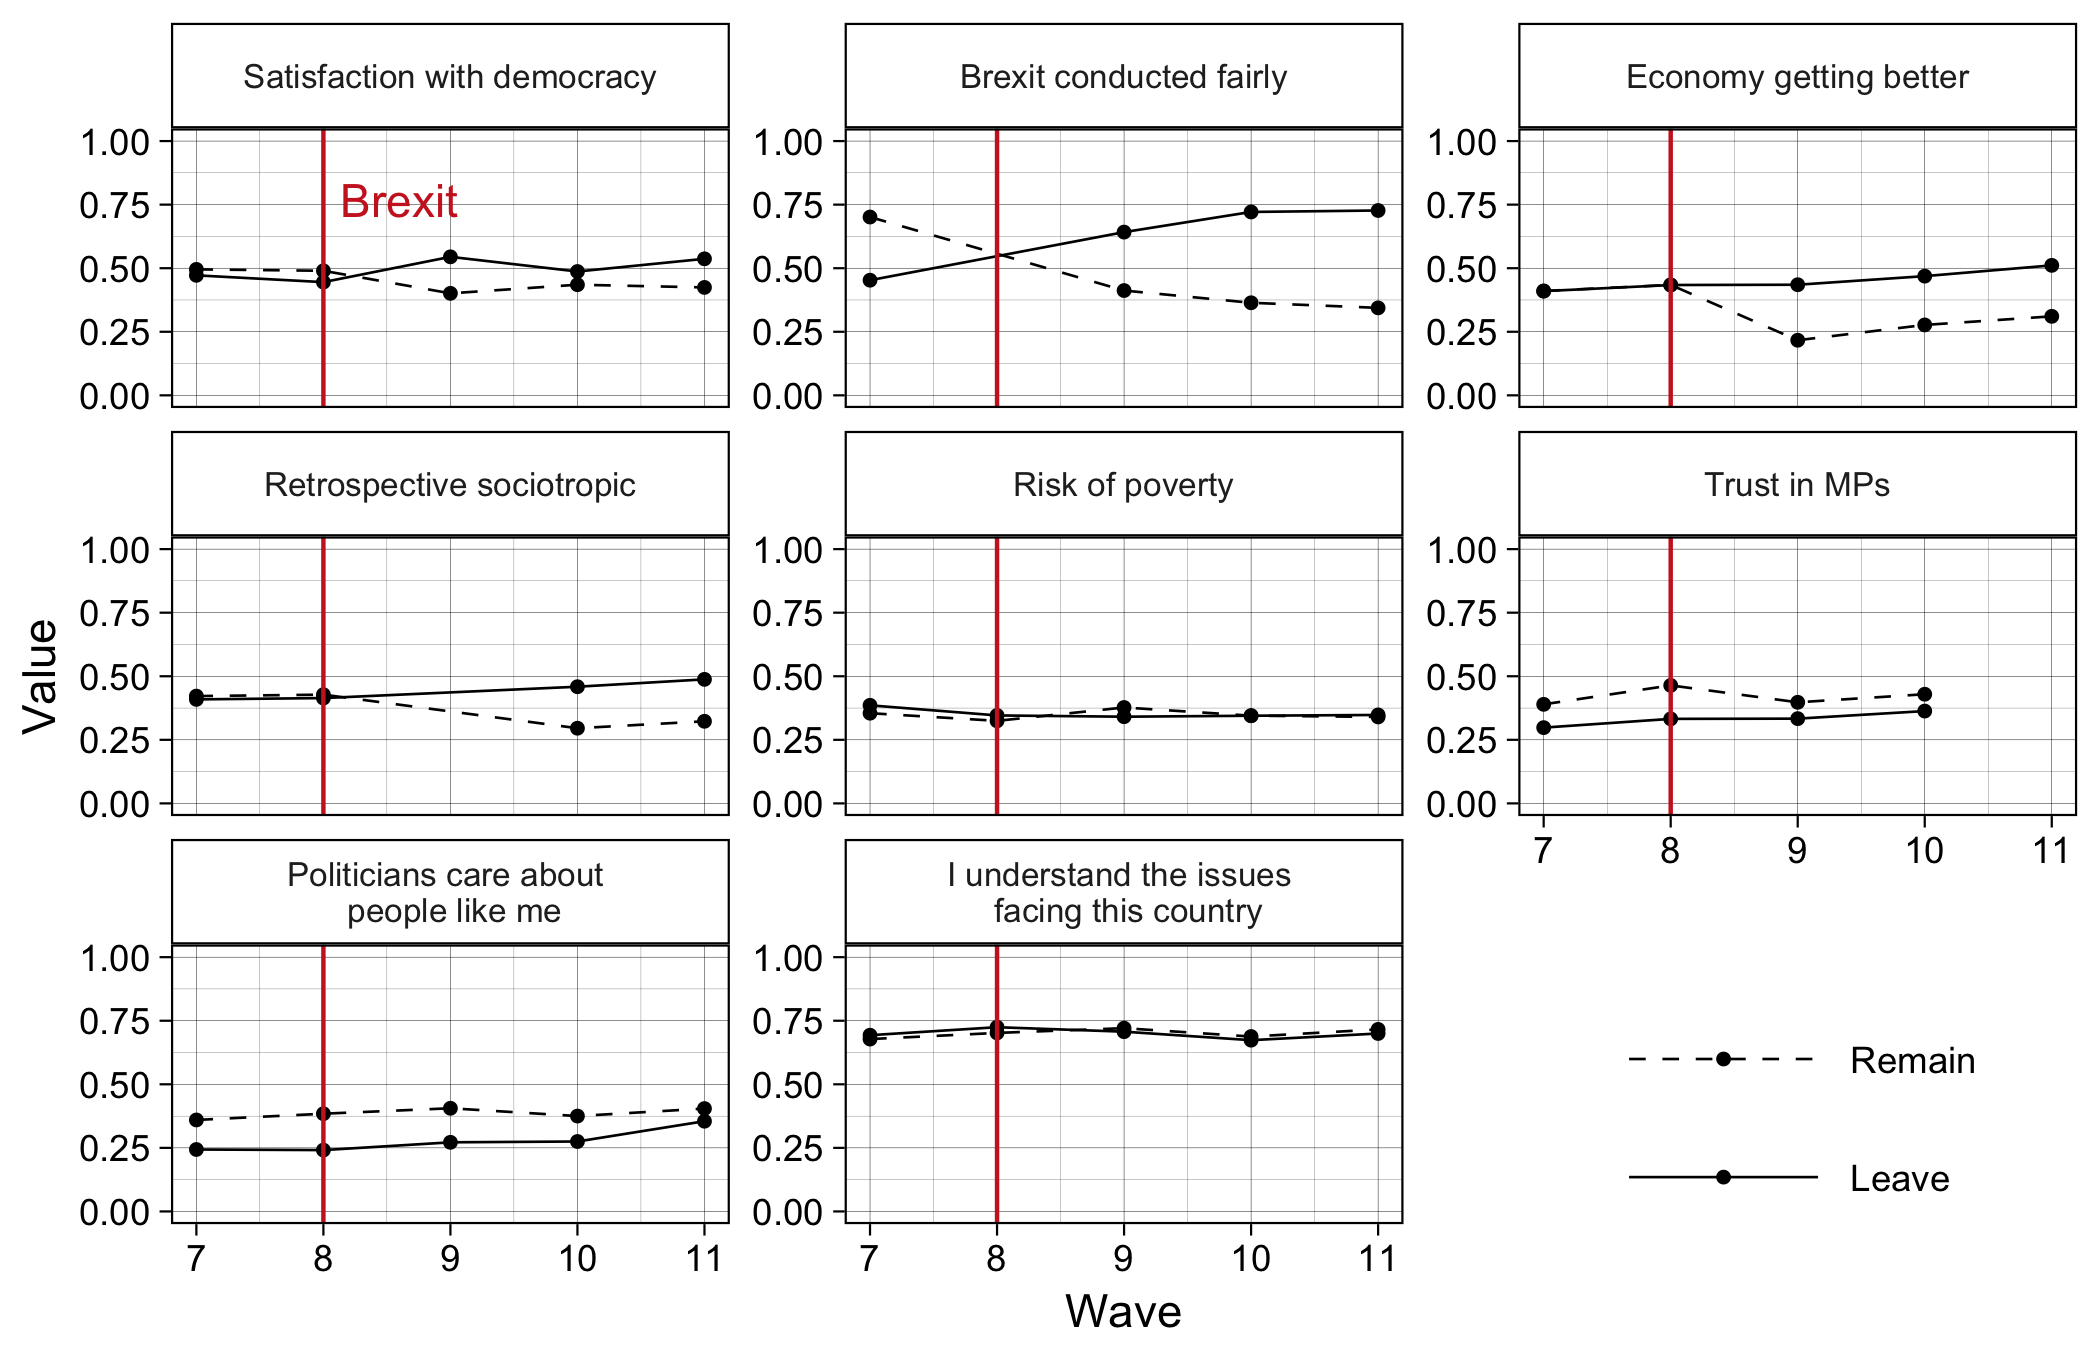
\includegraphics[scale=0.22]{plot_trends.png}
\label{fig:trends}
\end{figure}

\section{Data and Methods}

Data for this paper came from an internet panel study conducted from 2014-2017 as part of the British Election Study (BES) \parencite{bespanel}. These data are advantageous for examining the impact of the Brexit referendum on political attitudes because the same individuals were reinterviewed multiple times both before and after Brexit. The data were collected in thirteen waves spanning from February 2013 to June 9 2017. In each wave, around 30,000 respondents were interviewed. In total, only 17\% of respondents participated in all thirteen waves, though the vast majority completed at least two waves.\footnote{I have structured the data such that each observation is an individual during a given wave.} 

Because my primary interest is in changes in respondents' attitudes that occurred as a result of Brexit, I will draw on data collected from Wave 7 (April 14--May 4 2016) to Wave 11 (April 24--May 3). It is necessary to restrict the data in this way because of the general elections that were held on May 5, 2015 and June 8, 2017. These elections likely produced winner-loser gaps of their own, thus excluding them from the analysis will produce cleaner estimates of the winner-loser gap with respect to Brexit. 

To test the hypotheses discussed above, I estimate a number of OLS regressions where the key independent variables are winner-loser status and wave of interview. Winner-loser status is coded as a dummy variable where 0 indicates an intention to vote remain and 1 indicates an intention to vote leave, measured prior to the referendum, in Waves 7 and 8. I use an indicator for pre-Brexit vote intention instead of post-Brexit reported vote so as to reduce the possibility of post-treatment bias---that is, to eliminate the possibility that respondents change their reported vote choice as a consequence of the referendum.\footnote{The pre-Brexit vote intention questions asked the respondents if they were (a) planning to vote leave, (b) planning to vote remain, or (c) planning not vote. Another post-Brexit turnout question asked respondents if they voted in the referendum. Among respondents who answered both the pre-Brexit vote intention \textit{and} post-Brexit turnout questions, only 3.6 percent who reported that they would vote (remain or leave) indicated that they did not actually turn out. In other words, for pairwise complete cases, 96 percent of those who expressed a vote intention also said they voted in the referendum after the fact.} This indicator included 3 options: vote to leave the EU, vote to remain in the EU, and would not vote. As I am interested in the first two categories, I do not take respondents who reported that they would not vote in the Brexit referendum into account.

Wave of interview is also a binary variable that takes on a value of 1 for the post-Brexit wave of the survey. If the political attitudes of winners and losers change differentially from pre- to post-Brexit, we should expect to see a significant interaction between wave of interview and winner-loser status. In addition to these two primary independent variables and their interaction, I control for a number of factors known to be associated with political attitudes: income, age, age$^2$, education, ideology (left-right self-placement), attention to politics, party identification, and occupation. Additionally, because concerns over immigration and national identity clearly divided those in the leave and remain camps \parencite{hobolt2016brexit}, controls for both cultural and economic immigration attitudes are included. For variables that could plausibly change as a result of Brexit---ideology, income, attention to politics, party identification, and immigration attitudes---I use values from the pre-Brexit waves of the panel. All of these controls except for age and age$^2$ are recoded to range from 0 to 1, where wealthier, more right-wing, politically attentive, and more positive immigration attitudes take on higher values. Education is recoded as a dummy variable to indicate whether the respondent has received a post-secondary education. Lastly, occupation and party identification are represented by a set of dummy variables. To highlight the effect of the interaction between winner-loser status and Brexit, I do not present the effects of these controls in the main paper. Full models can be found in the Appendix \ref{measurmentwording}.

In each regression model, the dependent variable corresponds to one of the political attitudes or economic perceptions. Satisfaction with democracy is measured with a standard survey question that asks how satisfied respondents are with the way democracy works in the UK. To tap into questions of fairness, I combine two items that ask (1) how fairly the respondent thinks the Brexit referendum \textit{will be} conducted (asked in pre-Brexit waves) and (2) how fairly the respondent thinks the Brexit \textit{was} conducted (asked in post-Brexit waves). Sociotropic prospective economic evaluations are measured with a question that asks respondents the degree to which they think the economy is getting better or worse. Sociotropic retrospective economic evaluations are measured with a question that asked respondents how they think the general economic situation in the country has changed over the last 12 months. To gauge egocentric economic evaluations, I use a question in which respondents report the likelihood of not having enough money to cover daily living costs within the next 12 months.\footnote{While there are more standard measures of prospective sociotropic and egotropic evaluations in the BES---i.e. those commonly used in the economic voting literature, they were not asked in a sufficient number of panel waves and were thus not feasible to use.} To measure political trust, I use an item that asks respondents how much trust they have in MPs in general. Although this measure  taps into only one facet of political trust, it was the most relevant indicator available in the BES. Lastly, external efficacy is measured with a survey item that ask the respondent how much they agree with the statement ``politicians don't care what people like me think'' and internal efficacy is measured with the respondents' agreement with the statement ``I have a pretty good understanding of the important political issues facing our country.'' While the BES contained a number of measures related to internal and external efficacy, these two measures were the most relevant with respect to referendums.\footnote{For more reliable measures, it was suggested that I combine measures of efficacy to produce a more reliable measure. However, after running diagnostics on items for internal efficacy as well as external efficacy, I found low levels of internal consistency (Cronbach's alpha scores were all below 0.7). Because of this, I could not justify combining the measures.}

To allow for the comparison of regression coefficients across models, the dependent variables are all recoded to vary between 0 and 1. Details of their original scales can be found in Appendix D.

\begin{table}
\begin{center}
\caption{The short term impact of Brexit}
\setlength{\tabcolsep}{0.1em}
\scalebox{0.8}{
\begin{tabular}{l c c c c c c}
\hline 
\toprule[1.5pt]
\\[-1.8ex]
& \multicolumn{6}{c}{\textit{Dependent variable:}} \\
\\[-10pt]

&&&&&
\multirow{4}{70pt}{\centering Politicans care about people like me} &
\multirow{4}{70pt}{\centering I understand the issues facing the country} \\


& 
\multirow{3}{75pt}{\centering Satsisfaction with democracy} & 
\multirow{3}{75pt}{\centering Brexit conducted fairly} & 
\multirow{3}{70pt}{\centering Economy getting better} & & &  \\
 
 
&& \multirow{3}{60pt}[8pt]{\centering } & &
\multirow{3}{60pt}[8pt]{\centering Risk of poverty} &&
\\

\\[0pt]
 & (1) & (2) & (3) & (4) & (5) & (6) \\[3pt]
\cmidrule[1pt]{2-7}
\\[-12pt] 
Constant                         & $0.145^{*}$    & $0.606^{***}$  & $0.405^{***}$  & $0.311^{**}$   & $-0.010$       & $0.302^{***}$  \\
                                 & $(0.065)$      & $(0.079)$      & $(0.042)$      & $(0.097)$      & $(0.054)$      & $(0.031)$      \\
Brexit                           & $-0.086^{***}$ & $-0.242^{***}$ & $-0.198^{***}$ & $0.065^{***}$  & $0.021^{***}$  & $0.011^{**}$   \\
                                 & $(0.005)$      & $(0.007)$      & $(0.005)$      & $(0.009)$      & $(0.005)$      & $(0.003)$      \\
Leave                            & $-0.073^{***}$ & $-0.202^{***}$ & $-0.043^{***}$ & $0.031^{*}$    & $-0.074^{***}$ & $0.021^{***}$  \\
                                 & $(0.007)$      & $(0.008)$      & $(0.006)$      & $(0.014)$      & $(0.007)$      & $(0.005)$      \\
                                 Brexit X leave                   & $0.177^{***}$  & $0.409^{***}$  & $0.189^{***}$  & $-0.063^{***}$ & $0.002$        & $-0.023^{***}$ \\
                                 & $(0.007)$      & $(0.010)$      & $(0.007)$      & $(0.014)$      & $(0.006)$      & $(0.005)$      \\
\hline
R$^2$                            & 0.151          & 0.103          & 0.236          & 0.145          & 0.155          & 0.323          \\
Adj. R$^2$                       & 0.150          & 0.102          & 0.235          & 0.144          & 0.154          & 0.322          \\
Num. obs.                        & 28677          & 30707          & 28885          & 17530          & 29208          & 29299          \\
RMSE                             & 0.259          & 0.332          & 0.208          & 0.281          & 0.230          & 0.157          \\
\toprule[1.5pt]
\multicolumn{7}{l}{\scriptsize{$^{***}p<0.001$, $^{**}p<0.01$, $^*p<0.05$}} \\
\multicolumn{7}{l}{\multirow{3}{500pt}{\footnotesize{\textit{Notes:} Table entries are OLS regression coefficients. Standard errors in parentheses, clustered by respondent. Estimates for income, gender, age, education, left-right self placement, party identification, occupation, attention to politics and immigration attitudes not included (see Appendix \ref{appendixtable3}). All dependent variables range from zero to one.}}} \\
\end{tabular}
}
\label{table:coefficients}
\end{center}
\end{table}






\begin{table}[t]
\begin{center}
\caption{Six months after Brexit}
\setlength{\tabcolsep}{0.05em}
\scalebox{0.7}{
\begin{tabular}{l c c c c c c c c }
\hline 
\toprule[1.5pt]
\\[-1.8ex]
& \multicolumn{8}{c}{\textit{Dependent variable:}} \\
\\[-10pt]
&&&&&
\multirow{4}{60pt}{\centering } & 
\multirow{4}{75pt}{\centering } & 
\multirow{4}{60pt}{\centering Politicans care about people like me} &
\multirow{4}{70pt}{\centering I understand the issues facing the country} \\
& 
\multirow{3}{60pt}{\centering Satsisfaction with democracy} & 
\multirow{3}{60pt}{\centering Brexit conducted fairly} & 
\multirow{3}{50pt}{\centering Economy getting better} & 
\multirow{3}{60pt}{\centering Retro--spective sociotropic} & 
\multirow{3}{60pt}{\centering } & 
 & &  \\
&&& \multirow{3}{60pt}[8pt]{\centering } & &
\multirow{3}{60pt}[8pt]{\centering Risk of poverty} &
\multirow{3}{50pt}[8pt]{\centering Trust MPs}
&
\\
\\[0pt]
 & (1) & (2) & (3) & (4) & (5) & (6) & (7) & (8) \\[3pt]
\cmidrule[1pt]{2-9}
\\[-12pt] 
Constant                         & $0.074$        & $0.542^{***}$  & $0.368^{***}$  & $0.433^{***}$  & $0.517^{***}$  & $-0.160$       & $-0.011$       & $0.284^{***}$  \\
                                 & $(0.070)$      & $(0.079)$      & $(0.054)$      & $(0.054)$      & $(0.137)$      & $(0.094)$      & $(0.058)$      & $(0.040)$      \\
Brexit                           & $-0.050^{***}$ & $-0.283^{***}$ & $-0.134^{***}$ & $-0.119^{***}$ & $0.019^{*}$    & $-0.030^{**}$  & $-0.001$       & $-0.010^{*}$   \\
                                 & $(0.006)$      & $(0.008)$      & $(0.005)$      & $(0.008)$      & $(0.010)$      & $(0.011)$      & $(0.005)$      & $(0.004)$      \\
Leave                            & $-0.065^{***}$ & $-0.217^{***}$ & $-0.033^{***}$ & $-0.029^{**}$  & $0.028$        & $-0.076^{***}$ & $-0.077^{***}$ & $0.021^{***}$  \\
                                 & $(0.007)$      & $(0.008)$      & $(0.006)$      & $(0.011)$      & $(0.014)$      & $(0.017)$      & $(0.007)$      & $(0.005)$      \\
                                 Brexit X leave                   & $0.083^{***}$  & $0.517^{***}$  & $0.156^{***}$  & $0.129^{***}$  & $-0.012$       & $0.066^{***}$  & $0.027^{***}$  & $-0.028^{***}$ \\
                                 & $(0.008)$      & $(0.012)$      & $(0.007)$      & $(0.011)$      & $(0.014)$      & $(0.016)$      & $(0.007)$      & $(0.006)$      \\
\hline
R$^2$                            & 0.146          & 0.150          & 0.215          & 0.179          & 0.155          & 0.180          & 0.150          & 0.336          \\
Adj. R$^2$                       & 0.145          & 0.150          & 0.214          & 0.178          & 0.154          & 0.178          & 0.149          & 0.335          \\
Num. obs.                        & 25083          & 27268          & 25432          & 14523          & 14292          & 12567          & 25691          & 25755          \\
RMSE                             & 0.252          & 0.329          & 0.209          & 0.206          & 0.280          & 0.238          & 0.228          & 0.159          \\
\toprule[1.5pt]
\multicolumn{9}{l}{\scriptsize{$^{***}p<0.001$, $^{**}p<0.01$, $^*p<0.05$}} \\
\multicolumn{9}{l}{\multirow{3}{650pt}{\footnotesize{\textit{Notes:} Table entries are OLS regression coefficients. Standard errors in parentheses, clustered by respondent. Estimates for income, gender, age, education, left-right self placement, party identification, occupation, attention to politics and immigration attitudes not included (see Appendix \ref{appendixtable3}). All dependent variables range from zero to one.}}} \\
\end{tabular}}
\label{table:coefficients}
\end{center}
\end{table}




\begin{table}
\begin{center}
\caption{Ten months after Brexit}
\setlength{\tabcolsep}{0.05em}
\scalebox{0.7}{
\begin{tabular}{l c c c c c c c c }
\hline 
\toprule[1.5pt]
\\[-1.8ex]
& \multicolumn{8}{c}{\textit{Dependent variable:}} \\
\\[-10pt]
&&&&&
\multirow{4}{60pt}{\centering } & 
\multirow{4}{75pt}{\centering } & 
\multirow{4}{60pt}{\centering Politicans care about people like me} &
\multirow{4}{70pt}{\centering I understand the issues facing the country} \\
& 
\multirow{3}{60pt}{\centering Satsisfaction with democracy} & 
\multirow{3}{60pt}{\centering Brexit conducted fairly} & 
\multirow{3}{50pt}{\centering Economy getting better} & 
\multirow{3}{60pt}{\centering Retro--spective sociotropic} & 
\multirow{3}{60pt}{\centering } & 
 & &  \\
&&& \multirow{3}{60pt}[8pt]{\centering } & &
\multirow{3}{60pt}[8pt]{\centering Risk of poverty} &
\multirow{3}{50pt}[8pt]{\centering Trust MPs}
&
\\
\\[0pt]
 & (1) & (2) & (3) & (4) & (5) & (6) & (7) & (8) \\[3pt]
\cmidrule[1pt]{2-9}
\\[-12pt] 
Constant                         & $0.098$        & $0.380^{***}$  & $0.411^{***}$  & $0.580^{***}$  & $0.298^{**}$   & $-0.101$       & $0.024$        & $0.325^{***}$  \\
                                 & $(0.060)$      & $(0.063)$      & $(0.054)$      & $(0.066)$      & $(0.111)$      & $(0.089)$      & $(0.066)$      & $(0.030)$      \\
Brexit                           & $-0.052^{***}$ & $-0.311^{***}$ & $-0.108^{***}$ & $-0.098^{***}$ & $0.029^{**}$   & $-0.004$       & $0.030^{***}$  & $-0.001$       \\
                                 & $(0.006)$      & $(0.008)$      & $(0.005)$      & $(0.008)$      & $(0.010)$      & $(0.012)$      & $(0.005)$      & $(0.006)$      \\
Leave                            & $-0.074^{***}$ & $-0.216^{***}$ & $-0.041^{***}$ & $-0.047^{***}$ & $0.032^{*}$    & $-0.077^{***}$ & $-0.086^{***}$ & $0.019^{***}$  \\
                                 & $(0.007)$      & $(0.008)$      & $(0.006)$      & $(0.011)$      & $(0.014)$      & $(0.018)$      & $(0.007)$      & $(0.005)$      \\
Brexit X leave                   & $0.128^{***}$  & $0.546^{***}$  & $0.171^{***}$  & $0.133^{***}$  & $-0.015$       & $0.071^{***}$  & $0.068^{***}$  & $-0.016^{*}$   \\
                                 & $(0.008)$      & $(0.012)$      & $(0.007)$      & $(0.011)$      & $(0.014)$      & $(0.018)$      & $(0.007)$      & $(0.007)$      \\
\hline
R$^2$                            & 0.156          & 0.166          & 0.238          & 0.225          & 0.178          & 0.221          & 0.167          & 0.312          \\
Adj. R$^2$                       & 0.155          & 0.165          & 0.237          & 0.224          & 0.176          & 0.217          & 0.166          & 0.311          \\
Num. obs.                        & 25810          & 28045          & 26170          & 15250          & 15052          & 4775           & 26387          & 26477          \\
RMSE                             & 0.253          & 0.326          & 0.210          & 0.208          & 0.279          & 0.213          & 0.230          & 0.163          \\
\hline
\multicolumn{9}{l}{\scriptsize{$^{***}p<0.001$, $^{**}p<0.01$, $^*p<0.05$}} \\
\multicolumn{9}{l}{\multirow{3}{650pt}{\footnotesize{\textit{Notes:} Table entries are OLS regression coefficients. Standard errors in parentheses, clustered by respondent. Estimates for income, gender, age, education, left-right self placement, party identification, occupation, attention to politics and immigration attitudes not included (see Appendix \ref{appendixtable3}). All dependent variables range from zero to one.}}} \\
\end{tabular}}
\label{table:coefficients}
\end{center}
\end{table}



\section{Results}

Three sets of models are presented in this section to examine the effects of Brexit as well as the persistence of these effects into future waves. While all models draw on Wave 8 as a pre-Brexit baseline, I test for the same effects with progressively later waves of the survey. Accordingly, Table 1 draws on post-Brexit responses from Wave 9, administered for one month immediately after the referendum; Table 2 draws on responses from Wave 10, taken around six months after the referendum; and Table 3 uses responses from Wave 11, taken roughly 10 months after the referendum. The coefficients on the interaction between Brexit (post-Brexit waves of the survey) and Leave (winner-loser status) in each model represent the differential change between winners and losers from the pre- to post-Brexit period for the given dependent variable. These coefficients can be interpreted to represent the pre- to post-Brexit change associated with an intention to vote leave, relative to the effect for those who intended to vote remain \parencite{brambor2005understanding}. The baseline coefficient (Brexit) is thus attitudinal changes associated with Brexit on remainers.


I begin by examining the immediate shifts in attitudes associated with Brexit, presented in Table 1.\footnote{Table 1 excludes Trust in MPs and retrospective economic evaluations as these questions were not asked in Wave 9. In addition, perceptions of the fairness of the referendum draw on pre-Brexit responses from Wave 7, as this question was not asked in Wave 8.} For these regressions, I use responses from Wave 8 (just before the referendum) and Wave 9 (administered for one month immediately following the referendum). Strong differential effects can be observed with respect to satisfaction with democracy  (column 1, $\beta = 0.191$, $SE = 0.011$), prospective national economic evaluations (column 3, $\beta = 0.209$, $SE = 0.010$) and, most notably, perceptions that the referendum was conducted fairly (column 2, $\beta = 0.412$, $SE = 0.014$). The interaction terms in the models for personal economic evaluations (columns 4) and external efficacy (column 5) fail to reach conventional levels statistical significance. Although the effect of internal efficacy (column 6) is statistically significant, the substantive effects are negligible. Moreover, given the large number of observations in each model, statistical significance on this minimal effect is not entirely meaningful. 

From Table 2, it is clear that, to a large degree, the immediate effects of Brexit lasted into the second wave following the vote. While the differential effect of Brexit on satisfaction with democracy ($\beta = 0.101$, $SE = 0.011$) and prospective sociotropic economic evaluations ($\beta = 0.175$, $SE = 0.011$) decreased, perceptions of fairness \textit{increased} by over 10 points ($\beta = 0.529$, $SE = 0.016$). In addition, retrospective sociotropic economic evaluations and trust in MPs are introduced in Table 2, as Wave 10 was the first time these questions were asked after Brexit. While the effect of retrospective sociotropic evaluations ($\beta = 0.149$, $SE = 0.013$) largely mirrors that of prospective sociotropic evaluations, I find a relatively minor effect for trust in MPs ($\beta = 0.070$, $SE = 0.022$). 

Lastly, ten months after Brexit, it appears that the effects still persist for satisfaction with democracy ($\beta = 0.134$, $SE = 0.011$), prospective sociotropic economic evaluations ($\beta = 0.183$, $SE = 0.010$), retrospective economic evaluations ($\beta = 0.150$, $SE = 0.013$) and perception of the referendum's fairness ($\beta = 0.539$, $SE = 0.017$). 

While these results suggest a number of differential effects associated with Brexit, the coefficients on the interaction terms do not tell us the relative movement between winners and losers. As Figure \ref{fig:trends} suggests, the direction and strength of the Brexit's effect for Leavers relative to Remainers varies across different outcomes. In Tables 1, 2, and 3, the positive coefficients on satisfaction with democracy may reflect losers becoming less satisfied relative to winners, winners become more satisfied than winners, or both. Along these lines, it is necessary to plot the marginal effects of Brexit for both winners and losers in order to assess my hypotheses. To this end, Figure \ref{fig:marg} graphically illustrates the average marginal effects of Brexit accompanied by their 99\% confidence intervals. 

\begin{figure}[t]
\caption{OLS coefficients of Brexit on political attitudes by winner-loser status}
\hbox{\hspace{-0.5cm} 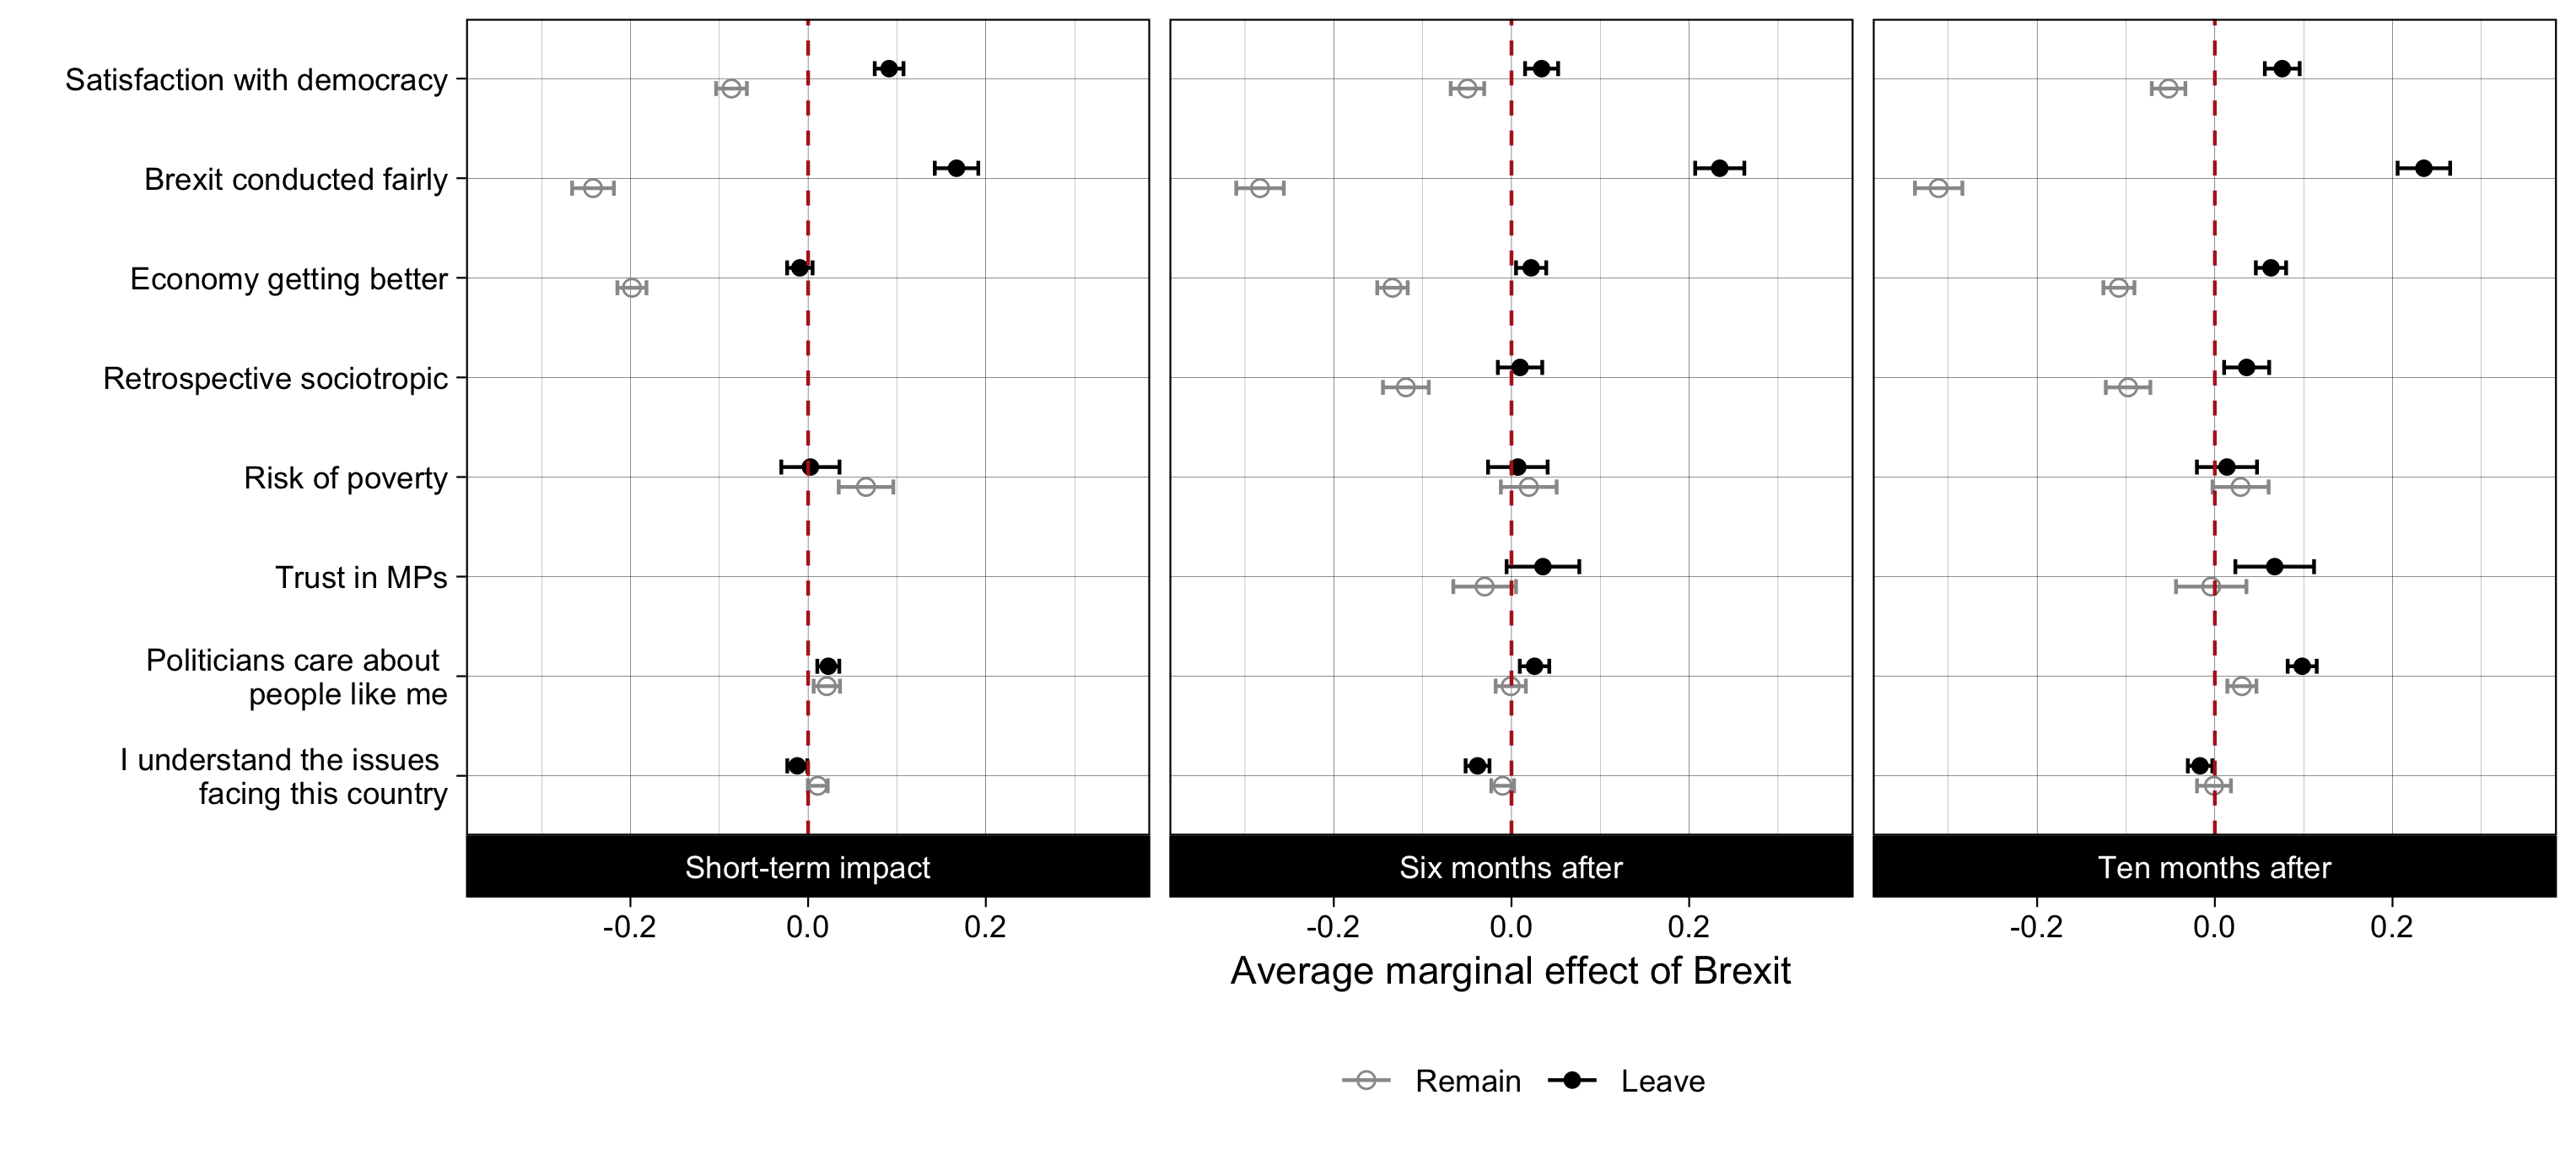
\includegraphics[scale=0.16]{margeff_plot.png}}
\label{fig:marg}
\end{figure}

The marginal effects of Brexit for winning and losing on satisfaction with the way democracy works in the UK largely confirm H1a and H1b---Brexit is associated with a moderate increase for winners and a roughly equivalent decrease for losers in satisfaction with democracy. While the effect is strongest immediately after the referendum, differences in democratic satisfaction appear to persist up to ten months after the referendum. This is in line with findings from the winner-loser gap literature that satisfaction with democracy is contingent on election outcomes \parencite{anderson2002winning, anderson2005losers, blais2007winning, bowler2002democracy}. Moreover, these results suggest that a similar process may be at play with respect to referendums. That said, it is difficult to say the exact mechanism that is producing this effect. Brexit was an extremely consequential decision accompanied by an intense campaign---the increase in democratic satisfaction associated with Brexit could plausibly be the result of emotional gratification, satisfaction with the policy implications of the result, or a combination of these and other factors. 

The most striking result from Figure \ref{fig:marg} is undoubtedly the divergence between how fairly respondents believed the referendum was conducted. That is, for respondents who reported that they would vote leave in the pre-Brexit period, the initial post-Brexit period is associated with a 16 point increase in perceptions of fairness, whereas those whose intention was to remain saw a 25 point decrease. Ten months after Brexit, this gap widens to a 23 percent increase for Leave respondents and a 33 percent decrease for Remain respondents. I take these changes as a confirmation of H2---outcome favourability appears to strongly shade perceptions of fairness. Indeed, although similar caveats about the unique political circumstances of Brexit as those above apply here, this finding is nonetheless consistent with works that find a legitimacy gap between the winners and losers of elections. It also suggests that, in the context of referendums---the Brexit referendum at least---outcome favourability may trump the enhanced decision-making influence afforded to citizens by this process \parencite{arnesen2017legitimacy}. While the mechanism once again is not clear-cut, the divergence in this relatively straightforward question is consistent with the notion that losers update their attitudes to restore consistency between their attitudes and behaviour.\footnote{This is not to suggest that these updated attitudes are necessarily wrong. Indeed, it is possible that those with a remain vote intention did expect the referendum to be conducted fairly before the referendum and updated their beliefs if it was not. If the recent allegations coming from whistleblowers who worked for the Leave campaign are accurate, this may be a reasonable reaction \url{http://www.cbc.ca/news/technology/chris-wylie-testify-uk-facebook-cambridge-analytica-1.4594668}.}

What implications do these results carry with respect to personal (H3e and H3f) and national (H3a--H3d) economic evaluations? The marginal effects of Brexit for winning and losing on both retrospective and prospective national economic evaluations lend support to H3b and H3c---the post-Brexit period accompanies a decrease in remainers' national economic evaluations. Leavers, on the other hand, did not seem to adjust their economic perceptions, which is surprising given that the pound fell dramatically immediately following the referendum. On the other hand, the effect of Brexit on personal economic evaluations in all 3 models is not statistically distinguishable from zero at the 99 percent level. That is, neither leavers nor remainers seem to update their perceived risk of unemployment and poverty after Brexit, disconfirming H3e and H3f. In short, these findings suggest that while Brexit winners and losers did not, on average, adjust their personal economic assessments to a large degree, the outcome of the Brexit referendum may have affected losers' perceptions of where the British economy was headed as well as how it had been performing. This is consistent with much of the literature on economic voting, where sociotropic economic considerations have consistently been found as more consequential to vote choice than egotropic considerations \parencite{lewis2013vp}. Obviously, my analysis is not about the determinants, but rather the \textit{consequences} of vote choice, though these findings are suggestive as to the type of economic evaluations most affected by referendums. Indeed, these findings are consistent with the notion that partisan predisposition---in this case, partisans of the Leave camp---impacts individuals' assessments the objective economy, perhaps even in the case of highly salient referendums like Brexit. 

Lastly, the post-Brexit period is associated in any meaningful way with improvements in measures of external and internal efficacy. Thus, H4a and H4b cannot be confirmed. A similar conclusion can be reached with respect to political trust. There appears to be little movement with respect to trust before and after the referendum for both Leave and Remain voters, disconfirming H4c. As mentioned earlier, there are not strong theoretical reasons to expect that a one-off referendum like Brexit would have the ability to transform strong predispositions like efficacy and trust, as participatory democratic theory predicts for contexts where direct democracy is more institutionalized. Indeed, the framework offered by participatory democratic theory may be inappropriate for an event like Brexit. 

\section{Discussion}

While it has been well-documented that conventional elections produce differential effects among winners and losers, this phenomena has received little attention in the context of referendums. This paper has gone some way toward expanding our understanding of the winner-loser gap to include non-conventional forms of democratic decision-making. Tracking individuals' political attitudes both before and after Brexit, I have found evidence that associating with the winning (Leave) or losing (Remain) of the referendum systematically impacted both democratic satisfaction as well as perceptions of the fairness of the decision-making process. With respect to the perceived legitimacy of referendum decisions, the reversal of attitudes between those who intended to vote Leave and Remain after Brexit suggests that outcome favourability, much like in conventional elections, is an important source of consent to referendum outcomes \parencite{nadeau1993accepting}.

Moreover, while it has been acknowledged that traditional forms of partisanship have a strong influence on perceptions of economic performance \parencite{wlezien1997economic, anderson2007end, bartels2002beyond}, this phenomena has received less attention in both the winner-loser gap and in the context of referendums. The results in this paper suggest an affinity toward the winning or losing side of the Brexit decision affects economic perceptions, and that these perceptions may have been affected by the outcome of the referendum itself. Indeed, those who intended to vote Remain prior to the Brexit vote became markedly less optimistic about where the British economy was heading as well as how it had been performing, while Leave voters largely maintained their pre-Brexit economic outlooks. 

Lastly, there is reason to doubt the magnitude with which Brexit referendum made citizens feel like their voices are being heard and that the government is responsive to their needs. In the context of conventional elections, \textcite[579]{craig2006winners} claim, this is especially likely when “candidates obscure the real issues by opting for either general platitudes or negative attacks, voters are unhappy with the electoral choices available to them, or doubts exist about whether the election itself was conducted in a fair and honest fashion.” There is little doubt that all three of these factors were at play during the Brexit referendum. For example, \textcite[50]{calhoun2016brexit} argues that the Brexit vote was ``grounded in nostalgia ... almost entirely negative and devoid of plans for an alternative future'' and that ``those who will have to live the longest with the consequences wanted a different choice.'' Moreover, while interest in participatory democracy as a solution for problems of political alienation and enthusiasm has grown among political scientists and policymakers, the Brexit referendum was clearly not proposed for these reasons. The primary motivation for holding a referendum on EU membership can be attributed to internal divisions within the Conservative party, rather than an earnest desire to engage citizens politically \parencite{hobolt2016public, moore2017policy, prosser2016calling}. Indeed, is likely that more meaningful and earnest attempts at engagement will be required for such an effect to take hold. As \textcite[154]{barber2003strong} notes,

\begin{quote}
political elites ``throw referenda at the people without providing adequate information, full debate, or prudent insulation from money and media pressures and then pillory them for their lack of judgement. They overwhelm the people with the least tractable problems of mass society---busing, inflation, tax structures, nuclear safety, right-to-work legislation, industrial waste disposal, environmental protection (all of which the representative elites have themselves have utterly failed to deal with)---and then carp at their uncertainty or indecisiveness or the simple-mindedness with they muddle through to a decision.'' 
\end{quote}

In this vein, the results from this paper suggest that the political attitudes changed most by the Brexit referendum were not those associated with greater citizen engagement in the political process, such as efficacy and trust, but rather those linked to whether or not one's desired outcome was achieved. 

While this paper offers some insights into how referendums can shape political attitudes, it also has several limitations. First, as has been emphasized throughout the paper, Brexit was not a normal referendum. This was a particularly important decision left to the people largely for political reasons. At the same time, this does not necessarily proscribe the generalizability of the findings: referendums are almost always held at the behest of representative elites and thus by definition will be held for political reasons. Moreover, as \textcite{prosser2016calling} notes, EU treaty referendums are usually held as a result of domestic political pressure. Brexit is not unique in this regard. That said, the most important and unresolved question to pose for future research is whether the effects found for Brexit hold for referendums held in other settings and over different questions.

Methodologically, it may be that the estimates in this paper are systematically influenced by factors unrelated to the winner-loser effect of Brexit. For instance, preceding the Brexit referendum was the 2015 general election, in which the Conservative party pledged a ``straight in-out referendum of the European Union by the end 2017'' parencite{conservative2015manifesto}. Another unexpected election was called early and came one year after the Brexit referendum in June of 2017 amidst leadership contests in both major parties. In addition, a variety of local elections were held concurrently with the 2015 and 2017 national elections as well as in 2016. Although the BES panel data was restricted to account for general and local elections, the possibility of bias does remain. Lastly, although the post-Brexit waves of the survey stretch until almost a year after the referendum, it is hard deliberate on long-term impact. This is true not only because of the limited scope of the panel, but also because, as more elections and perhaps more referendums occur, it will be increasingly difficult to trace attitudinal changes back to Brexit. 

Turning to the implications of the findings, while a large body of literature has explored this question in contexts where direct democracy is a standard feature of the political system, less attention has been paid to the impact of referendums in contexts where they occur less frequently. That said, it is important to understand how sporadic yet extremely consequential referendums such as Brexit affect citizens. This is especially true amidst the rise of populism in advanced industrial democracies as virtually all these call for the increased use of referendums or other forms of plebiscitary democracy \parencite{mudde2007populist}. Thus, understanding the impact of referendums on citizens political support, especially among the losers of these processes, has become an increasingly relevant line of inquiry.  

\singlespacing
\appendix

\section*{Appendix}

\section{Panel Data Structure}

These are the number of waves in the panel study as well as when they were conducted. As can be seen, Brexit is sandwiched between two elections, which might produce their own winner-loser effect or affect political attitudes in some other way. For this reason, the data are contrained to include only Waves 7 through 11. It is my hope that this will provide cleaner estimates of the changes associated with Brexit.

\begin{center}
\scalebox{0.65}{
\begin{tabular}{lllllllllllll}
\toprule[1.5pt]
 Wave 1 & Wave 2 & Wave 3 & Wave 4 & Wave 5 & Wave 6 & Wave 7 & Wave 8 & Wave 9 & Wave 10 & Wave 11 & Wave 12 & Wave 13 \\ 
\toprule[0.8pt]
 Feb 20-- & May 22-- & Sept 19-- & Mar 4-- & Mar 31-- & May 8-- & April 14-- & May 6-- & Jun 24-- & Nov 24-- & April 24-- & May 5-- & June 9-- \\
 Mar 9    & June 25  & Oct 17    & Mar 30  & May 6    & May 26  & May 4      & June 22 & July 4   & Dec 12 & May 3 & June 7 & June 23 \\ 
  2014 & 2014 & 2014 & 2015 & 2015 & 2015 & 2016 & 2016 & 2016 & 2016 & 2017 & 2017 & 2017 \\ 
\toprule[0.8pt]
 &  & & &Pre-     & Post-    & & Pre-   & Post-   &   & & Pre-     & Post-\\
 &  & & &election & election & & Brexit & Brexit &  & & election & election\\ 
\toprule[1.5pt]
\end{tabular}}
\end{center}

\section{Marginal effects}

These are the values for the marginal effects plotted in Figure 1. I must credit Frederik Hjorth for the code used to create these values (\texttt{https://gist.github.com/fghjorth/45c81a15f40660bc2852}). I use the function \texttt{interaction\_plot\_binary} in conjunction with \texttt{cluster.vcov} function from the \texttt{multiwayvcov} package to produce marginal effects with cluster robust confidence intervals.

\footnotesize
\begin{center}
\begin{longtable}{lcccccc}
\toprule[1.5pt]
  & \multicolumn{3}{c}{Remain} & \multicolumn{3}{c}{Leave} \\
  \cmidrule[1pt](lr){2-4} \cmidrule[1pt](lr){5-7}
Dependent variable & Lower  & Marg.  & Upper  & Lower & Marg.  & Upper  \\
 &  CI &  Effect & CI &  CI & Effect & CI \\ 
\toprule[1pt]
& \multicolumn{6}{c}{\textbf{Short-term impact of Brexit}} \\[3pt]
Sastisfaction with Democracy in the UK & -0.12 & -0.09 & -0.07 & 0.08 & 0.10 & 0.11 \\ 
How fairly will/was Brexit (be) conducted? & -0.28 & -0.25 & -0.22 & 0.14 & 0.16 & 0.19 \\ [3pt]
The economy is getting worse-better & -0.24 & -0.22 & -0.20 & -0.03 & -0.01 & 0.01 \\\\[3pt] 
\multirow{2}{200pt}{Likelihood of not having enough to cover daily living costs during next 12 months} & 0.01 & 0.05 & 0.09 & -0.02 & 0.02 & 0.06 \\ \\ 
\\[3pt]
Politicians don't care what people like me think & -0.00 & 0.02 & 0.04 & 0.01 & 0.02 & 0.04 \\[3pt] 
\multirow{2}{200pt}{I have a pretty good understanding of the important political issues facing our country} & 0.01 & 0.02 & 0.03 & -0.02 & -0.01 & 0.00 \\  
\\[3pt]
   \\[-7pt]

\toprule[1pt]
& \multicolumn{6}{c}{\textbf{Six months after Brexit}} \\[3pt]
Sastisfaction with Democracy in the UK & -0.08 & -0.06 & -0.03 & 0.03 & 0.05 & 0.06 \\ 
How fairly will/was Brexit (be) conducted? & -0.33 & -0.30 & -0.27 & 0.20 & 0.23 & 0.26 \\ 
The economy is getting worse-better & -0.17 & -0.15 & -0.13 & 0.01 & 0.03 & 0.05 \\[3pt] 
The economy has gotten worse-better & -0.15 & -0.12 & -0.10 & 0.00 & 0.02 & 0.05 \\[3pt] 
\multirow{2}{200pt}{Likelihood of not having enough to cover daily living costs during next 12 months} & -0.02 & 0.01 & 0.05 & -0.02 & 0.02 & 0.06 \\ 
\\[3pt]
\multirow{2}{200pt}{How much trust do you have in Members of Parliament in general?} & -0.06 & -0.03 & 0.01 & 0.00 & 0.05 & 0.09 \\ 
\\[3pt]
Politicians don't care what people like me think & 0.00 & 0.02 & 0.04 & 0.09 & 0.11 & 0.12 \\[3pt] 
\multirow{2}{200pt}{I have a pretty good understanding of the important political issues facing our country} & -0.02 & -0.00 & 0.01 & -0.05 & -0.04 & -0.02 \\ 
\\[3pt]
   \\[-7pt]

\toprule[1pt]
& \multicolumn{6}{c}{\textbf{Ten months after Brexit}} \\[3pt]
Sastisfaction with Democracy in the UK & -0.07 & -0.05 & -0.03 & 0.06 & 0.08 & 0.10 \\[3pt] 
How fairly will/was Brexit (be) conducted? & -0.33 & -0.30 & -0.28 & 0.20 & 0.23 & 0.27 \\[3pt]
The economy is getting worse-better & -0.14 & -0.12 & -0.10 & 0.05 & 0.07 & 0.08 \\[3pt] 
The economy has gotten worse-better & -0.12 & -0.10 & -0.08 & 0.03 & 0.05 & 0.07 \\[3pt] 
\multirow{2}{200pt}{Likelihood of not having enough to cover daily living costs during next 12 months} & -0.01 & 0.02 & 0.06 & -0.02 & 0.02 & 0.05 \\ 
\\[3pt]
\multirow{2}{200pt}{How much trust do you have in Members of Parliament in general?} & -0.03 & 0.01 & 0.05 & 0.02 & 0.06 & 0.11 \\ 
\\[3pt]
Politicians don't care what people like me think & 0.00 & 0.02 & 0.04 & 0.09 & 0.11 & 0.12 \\[3pt] 
\multirow{2}{200pt}{I have a pretty good understanding of the important political issues facing our country} & -0.02 & 0.00 & 0.02 & -0.03 & -0.01 & 0.00 \\ 
\\[3pt]
   \\[-7pt]
How fairly will/was Brexit (be) conducted? & -0.30 & -0.28 & -0.26 & 0.20 & 0.22 & 0.24 \\ 

\toprule[1.5pt]



\end{longtable}
\end{center}

\section{Depedent variables by panel wave}
As mentioned above, not all dependent variables were asked in all surveys. Find below a table which shows which dependent variables were asked in which waves. 

\begin{center}
\scriptsize
\begin{longtable}{llllll}
\toprule[1.5pt]
Dependent variable & Wave 7 & Wave 8 & Wave 9 & Wave 10 & Wave 11 \\ 
\toprule[1pt]
Sastisfaction with Democracy in the UK & $\times$ & $\times$ & $\times$ & $\times$ & $\times$ \\ 
 \\[-4pt]
Sastisfaction with Democracy in the EU & $\times$ & $\times$ & $\times$ & $\times$ &  \\ 
 \\[-4pt]
Politicians don't care what people like me think & $\times$ & $\times$ & $\times$ & $\times$ & $\times$ \\ 
 \\[-4pt]
It doesn't matter which party is in power & $\times$ &  & $\times$ & $\times$ & $\times$ \\ 
 \\[-4pt]
It is often difficult for me to understand what  & $\times$ &  & $\times$ & $\times$ & $\times$ \\
is going on in government and politics &&&&& \\
 \\[-4pt]
I have a pretty good understanding of the & $\times$ & $\times$ & $\times$ & $\times$ & $\times$ \\ 
important political issues facing our country &&&&& \\ 
 \\[-4pt]
Likelihood of being out of a job and & $\times$ & $\times$ & $\times$ & $\times$ & $\times$ \\ 
looking for work during next 12 months &&&&& \\
 \\[-4pt]
The economy is getting worse-better & $\times$ & $\times$ & $\times$ & $\times$ & $\times$ \\ 
 \\[-4pt]
Likelihood of not having enough to cover daily  & $\times$ & $\times$ & $\times$ & $\times$ & $\times$ \\ 
living costs during next 12 months &&&&& \\ 
 \\[-4pt]
How much trust do you have in Members of Parliament in & $\times$ & $\times$ & $\times$ & $\times$ &  \\ 
in general? &&&&& \\
 \\[-4pt]
How fairly will/was Brexit (be) conducted? & $\times$ &  & $\times$ & $\times$ & $\times$ \\ 
\toprule[1.5pt]
\end{longtable}
\end{center}

\section{Variables measurement and wording} \label{measurmentwording}

All of the dependent variables and most of the independent variables in this paper were recoded to range from 0 to 1 for comparable interpretation. These are the original measures of the dependent variables. The final version of this paper will also detail the measurement of the independent variables. Until then, please consult the BES codebook \url{http://www.britishelectionstudy.com/wp-content/uploads/2017/07/Bes\_wave13Documentation\_V1.0.pdf}. 

\scriptsize
\begin{center}
\begin{longtable}{lll}
\toprule[1pt]
Dependent variable & Range & Wording \\
\toprule[1pt]
On the whole, how satisfied or dissatisfied are you with the way that democracy  & 1--4 & Very dissatisfied --  \\
works in the UK && very satisfied\\
 \\[-4pt]
On the whole, how satisfied or dissatisfied are you with the way that democracy  & 1--4 & Very dissatisfied --  \\
works in EU && very satisfied\\
 \\[-4pt]
How fairly do you expect the EU referendum to be conducted? & 1--5 & Conducted fairly --  \\
&& conducted unfairly\\
 \\[-4pt]
Do you think that {[}the economy is{]} getting better, getting worse or staying  & 1--5 & Getting a lot worse --  \\
about the same? && getting a lot better\\
 \\[-4pt]
During the next 12 months, how likely or unlikely is it that you will be out of  & 1--5 & Very unlikely --  \\
a job and looking for work?&& very likely\\
 \\[-4pt]
During the next 12 months, how likely or unlikely is it that there will be times  & 1--5 & Very unlikely -- \\
when you don’t have enough money to cover your day to day living costs & & very likely \\
 \\[-4pt]
How much trust do you have in Members of Parliament in general? & 1-7 & No trust --  \\
 &  &  a great deal of trust \\
 \\[-4pt]
Politicians don’t care what people like me think & 1--5 & Strongly disagree --  \\
 &  &  strongly agree\\
 \\[-4pt]
It doesn’t matter which political party is in power & 1--5 & Strongly disagree -- \\
 &  &  strongly agree\\
 \\[-4pt]
It is often difficult for me to understand what is going on in government  & 1--5 & Strongly disagree -- \\
and politics && strongly agree\\
 \\[-4pt]
I have a pretty good understanding of the important political issues facing  & 1--5 & Strongly disagree --\\
our country && strongly agree\\
\toprule[1.5pt]
\end{longtable}
\end{center}


\section{Table 1 with full controls} \label{appendixtable1}

\begin{table}[H]
\begin{center}
\caption{The short term impact of Brexit}
\setlength{\tabcolsep}{0.1em}
\scalebox{0.7}{
\begin{tabular}{l c c c c c c}
\hline 
\toprule[1.5pt]
\\[-1.8ex]
& \multicolumn{6}{c}{\textit{Dependent variable:}} \\
\\[-10pt]

&&&&&
\multirow{4}{70pt}{\centering Politicans care about people like me} &
\multirow{4}{70pt}{\centering I understand the issues facing the country} \\


& 
\multirow{3}{75pt}{\centering Satsisfaction with democracy} & 
\multirow{3}{75pt}{\centering Brexit conducted fairly} & 
\multirow{3}{70pt}{\centering Economy getting better} & & &  \\
 
 
&& \multirow{3}{60pt}[8pt]{\centering } & &
\multirow{3}{60pt}[8pt]{\centering Risk of poverty} &&
\\

\\[0pt]
 & (1) & (2) & (3) & (4) & (5) & (6) \\[3pt]
\cmidrule[1pt]{2-7}
\\[-12pt] 

Constant                         & $0.145^{*}$    & $0.606^{***}$  & $0.405^{***}$  & $0.311^{**}$   & $-0.010$       & $0.302^{***}$  \\
                                 & $(0.065)$      & $(0.079)$      & $(0.042)$      & $(0.097)$      & $(0.054)$      & $(0.031)$      \\
Brexit                           & $-0.086^{***}$ & $-0.242^{***}$ & $-0.198^{***}$ & $0.065^{***}$  & $0.021^{***}$  & $0.011^{**}$   \\
                                 & $(0.005)$      & $(0.007)$      & $(0.005)$      & $(0.009)$      & $(0.005)$      & $(0.003)$      \\
Leave                            & $-0.073^{***}$ & $-0.202^{***}$ & $-0.043^{***}$ & $0.031^{*}$    & $-0.074^{***}$ & $0.021^{***}$  \\
                                 & $(0.007)$      & $(0.008)$      & $(0.006)$      & $(0.014)$      & $(0.007)$      & $(0.005)$      \\
Income                           & $0.036^{**}$   & $0.057^{***}$  & $0.014$        & $-0.325^{***}$ & $0.080^{***}$  & $0.036^{***}$  \\
                                 & $(0.012)$      & $(0.013)$      & $(0.009)$      & $(0.016)$      & $(0.011)$      & $(0.007)$      \\
Age                              & $0.001$        & $0.001$        & $-0.002^{*}$   & $0.008^{***}$  & $-0.002$       & $0.003^{***}$  \\
                                 & $(0.001)$      & $(0.001)$      & $(0.001)$      & $(0.002)$      & $(0.001)$      & $(0.001)$      \\
Age$^2$                            & $-0.000$       & $-0.000$       & $0.000$        & $-0.000^{***}$ & $0.000$        & $-0.000^{***}$ \\
                                 & $(0.000)$      & $(0.000)$      & $(0.000)$      & $(0.000)$      & $(0.000)$      & $(0.000)$      \\
Education                        & $-0.021^{***}$ & $0.012$        & $-0.011^{*}$   & $-0.030^{***}$ & $0.023^{***}$  & $0.016^{***}$  \\
                                 & $(0.006)$      & $(0.007)$      & $(0.005)$      & $(0.008)$      & $(0.006)$      & $(0.004)$      \\
Ideology                         & $0.291^{***}$  & $0.020$        & $0.225^{***}$  & $-0.091^{***}$ & $0.099^{***}$  & $-0.030^{*}$   \\
                                 & $(0.020)$      & $(0.021)$      & $(0.016)$      & $(0.025)$      & $(0.016)$      & $(0.013)$      \\
Gender                           & $0.019^{***}$  & $0.016^{**}$   & $-0.020^{***}$ & $0.037^{***}$  & $0.024^{***}$  & $-0.026^{***}$ \\
                                 & $(0.005)$      & $(0.006)$      & $(0.004)$      & $(0.007)$      & $(0.005)$      & $(0.003)$      \\
Scotland                         & $-0.015$       & $0.024^{**}$   & $0.006$        & $-0.033^{**}$  & $0.029^{***}$  & $-0.008$       \\
                                 & $(0.009)$      & $(0.009)$      & $(0.007)$      & $(0.011)$      & $(0.008)$      & $(0.005)$      \\
Wales                            & $0.003$        & $0.006$        & $-0.004$       & $0.002$        & $0.023^{**}$   & $0.010^{*}$    \\
                                 & $(0.010)$      & $(0.011)$      & $(0.007)$      & $(0.012)$      & $(0.008)$      & $(0.005)$      \\
Conservative                     & $0.282^{***}$  & $0.074$        & $0.105^{**}$   & $0.058$        & $0.193^{***}$  & $-0.009$       \\
                                 & $(0.055)$      & $(0.068)$      & $(0.033)$      & $(0.087)$      & $(0.041)$      & $(0.023)$      \\
Green                            & $0.086$        & $-0.037$       & $-0.022$       & $0.046$        & $0.027$        & $-0.013$       \\
                                 & $(0.058)$      & $(0.072)$      & $(0.036)$      & $(0.090)$      & $(0.045)$      & $(0.025)$      \\
Labour                           & $0.232^{***}$  & $0.011$        & $0.010$        & $0.121$        & $0.086^{*}$    & $-0.028$       \\
                                 & $(0.056)$      & $(0.068)$      & $(0.033)$      & $(0.087)$      & $(0.041)$      & $(0.023)$      \\
Liberal Democrat                 & $0.192^{***}$  & $0.026$        & $0.032$        & $0.070$        & $0.132^{**}$   & $-0.011$       \\
                                 & $(0.056)$      & $(0.069)$      & $(0.034)$      & $(0.088)$      & $(0.043)$      & $(0.024)$      \\
Other/don't know/none            & $0.168^{**}$   & $0.010$        & $0.020$        & $0.097$        & $0.089^{*}$    & $-0.021$       \\
                                 & $(0.056)$      & $(0.068)$      & $(0.033)$      & $(0.087)$      & $(0.041)$      & $(0.023)$      \\
Plaid Cyrmu                      & $0.096$        & $-0.030$       & $0.015$        & $0.085$        & $0.123^{*}$    & $-0.009$       \\
                                 & $(0.063)$      & $(0.075)$      & $(0.040)$      & $(0.097)$      & $(0.051)$      & $(0.028)$      \\
Scottish National Party          & $0.055$        & $-0.065$       & $-0.021$       & $0.112$        & $0.093^{*}$    & $-0.015$       \\
                                 & $(0.058)$      & $(0.070)$      & $(0.036)$      & $(0.089)$      & $(0.043)$      & $(0.024)$      \\
UKIP                             & $0.145^{**}$   & $-0.035$       & $-0.001$       & $0.100$        & $0.085^{*}$    & $0.009$        \\
                                 & $(0.056)$      & $(0.069)$      & $(0.033)$      & $(0.088)$      & $(0.042)$      & $(0.023)$      \\
Routine/semi-routine occupation  & $0.004$        & $-0.001$       & $0.010^{*}$    & $0.025^{**}$   & $-0.006$       & $-0.004$       \\
                                 & $(0.007)$      & $(0.007)$      & $(0.005)$      & $(0.009)$      & $(0.006)$      & $(0.004)$      \\
Attention to politics            & $-0.111^{***}$ & $-0.105^{***}$ & $-0.040^{**}$  & $0.059^{**}$   & $0.099^{***}$  & $0.567^{***}$  \\
                                 & $(0.016)$      & $(0.017)$      & $(0.013)$      & $(0.022)$      & $(0.013)$      & $(0.011)$      \\
Immigration attitudes (cultural) & $0.075^{***}$  & $0.026$        & $-0.012$       & $0.015$        & $0.089^{***}$  & $-0.030^{**}$  \\
                                 & $(0.019)$      & $(0.019)$      & $(0.014)$      & $(0.026)$      & $(0.019)$      & $(0.011)$      \\
Immigration attitudes (economic) & $-0.013$       & $-0.000$       & $0.030$        & $-0.057^{*}$   & $0.080^{***}$  & $0.014$        \\
                                 & $(0.020)$      & $(0.021)$      & $(0.015)$      & $(0.027)$      & $(0.022)$      & $(0.012)$      \\
Brexit X leave                   & $0.177^{***}$  & $0.409^{***}$  & $0.189^{***}$  & $-0.063^{***}$ & $0.002$        & $-0.023^{***}$ \\
                                 & $(0.007)$      & $(0.010)$      & $(0.007)$      & $(0.014)$      & $(0.006)$      & $(0.005)$      \\
\hline
R$^2$                            & 0.151          & 0.103          & 0.236          & 0.145          & 0.155          & 0.323          \\
Adj. R$^2$                       & 0.150          & 0.102          & 0.235          & 0.144          & 0.154          & 0.322          \\
Num. obs.                        & 28677          & 30707          & 28885          & 17530          & 29208          & 29299          \\
RMSE                             & 0.259          & 0.332          & 0.208          & 0.281          & 0.230          & 0.157          \\
\hline
\multicolumn{7}{l}{\scriptsize{$^{***}p<0.001$, $^{**}p<0.01$, $^*p<0.05$}}
\end{tabular}
}
\end{center}
\end{table}

\section{Table 2 with full controls} \label{appendixtable2}

\begin{table}[H]
\begin{center}
\caption{Six months after Brexit}
\setlength{\tabcolsep}{0.05em}
\scalebox{0.6}{
\begin{tabular}{l c c c c c c c c }
\hline 
\toprule[1.5pt]
\\[-1.8ex]
& \multicolumn{8}{c}{\textit{Dependent variable:}} \\
\\[-10pt]
&&&&&
\multirow{4}{60pt}{\centering } & 
\multirow{4}{75pt}{\centering } & 
\multirow{4}{60pt}{\centering Politicans care about people like me} &
\multirow{4}{70pt}{\centering I understand the issues facing the country} \\
& 
\multirow{3}{60pt}{\centering Satsisfaction with democracy} & 
\multirow{3}{60pt}{\centering Brexit conducted fairly} & 
\multirow{3}{50pt}{\centering Economy getting better} & 
\multirow{3}{60pt}{\centering Retro--spective sociotropic} & 
\multirow{3}{60pt}{\centering } & 
 & &  \\
&&& \multirow{3}{60pt}[8pt]{\centering } & &
\multirow{3}{60pt}[8pt]{\centering Risk of poverty} &
\multirow{3}{50pt}[8pt]{\centering Trust MPs}
&
\\
\\[0pt]
 & (1) & (2) & (3) & (4) & (5) & (6) & (7) & (8) \\[3pt]
\cmidrule[1pt]{2-9}
\\[-12pt] 
Constant                         & $0.074$        & $0.542^{***}$  & $0.368^{***}$  & $0.433^{***}$  & $0.517^{***}$  & $-0.160$       & $-0.011$       & $0.284^{***}$  \\
                                 & $(0.070)$      & $(0.079)$      & $(0.054)$      & $(0.054)$      & $(0.137)$      & $(0.094)$      & $(0.058)$      & $(0.040)$      \\
Brexit                           & $-0.050^{***}$ & $-0.283^{***}$ & $-0.134^{***}$ & $-0.119^{***}$ & $0.019^{*}$    & $-0.030^{**}$  & $-0.001$       & $-0.010^{*}$   \\
                                 & $(0.006)$      & $(0.008)$      & $(0.005)$      & $(0.008)$      & $(0.010)$      & $(0.011)$      & $(0.005)$      & $(0.004)$      \\
Leave                            & $-0.065^{***}$ & $-0.217^{***}$ & $-0.033^{***}$ & $-0.029^{**}$  & $0.028$        & $-0.076^{***}$ & $-0.077^{***}$ & $0.021^{***}$  \\
                                 & $(0.007)$      & $(0.008)$      & $(0.006)$      & $(0.011)$      & $(0.014)$      & $(0.017)$      & $(0.007)$      & $(0.005)$      \\
Income                           & $0.046^{***}$  & $0.061^{***}$  & $0.030^{**}$   & $0.025$        & $-0.321^{***}$ & $0.038^{*}$    & $0.080^{***}$  & $0.026^{***}$  \\
                                 & $(0.012)$      & $(0.014)$      & $(0.011)$      & $(0.014)$      & $(0.017)$      & $(0.016)$      & $(0.011)$      & $(0.007)$      \\
Age                              & $0.000$        & $0.002$        & $-0.003^{**}$  & $-0.003$       & $0.009^{***}$  & $-0.003$       & $-0.002$       & $0.004^{***}$  \\
                                 & $(0.001)$      & $(0.001)$      & $(0.001)$      & $(0.001)$      & $(0.002)$      & $(0.002)$      & $(0.001)$      & $(0.001)$      \\
Age$^2$                            & $-0.000$       & $-0.000$       & $0.000$        & $0.000$        & $-0.000^{***}$ & $0.000^{*}$    & $0.000$        & $-0.000^{***}$ \\
                                 & $(0.000)$      & $(0.000)$      & $(0.000)$      & $(0.000)$      & $(0.000)$      & $(0.000)$      & $(0.000)$      & $(0.000)$      \\
Education                        & $-0.014^{*}$   & $0.008$        & $-0.006$       & $-0.002$       & $-0.046^{***}$ & $-0.009$       & $0.018^{**}$   & $0.015^{***}$  \\
                                 & $(0.006)$      & $(0.007)$      & $(0.005)$      & $(0.007)$      & $(0.009)$      & $(0.008)$      & $(0.006)$      & $(0.004)$      \\
Ideology                         & $0.321^{***}$  & $0.071^{**}$   & $0.249^{***}$  & $0.205^{***}$  & $-0.087^{***}$ & $0.222^{***}$  & $0.110^{***}$  & $-0.033^{*}$   \\
                                 & $(0.021)$      & $(0.022)$      & $(0.018)$      & $(0.024)$      & $(0.026)$      & $(0.027)$      & $(0.017)$      & $(0.013)$      \\
Gender                           & $0.022^{***}$  & $0.026^{***}$  & $-0.018^{***}$ & $-0.015^{**}$  & $0.014$        & $0.025^{***}$  & $0.018^{***}$  & $-0.030^{***}$ \\
                                 & $(0.005)$      & $(0.006)$      & $(0.005)$      & $(0.006)$      & $(0.008)$      & $(0.007)$      & $(0.005)$      & $(0.003)$      \\
Scotland                         & $-0.012$       & $0.049^{***}$  & $0.005$        & $0.006$        & $-0.041^{***}$ & $0.005$        & $0.022^{**}$   & $-0.006$       \\
                                 & $(0.009)$      & $(0.010)$      & $(0.007)$      & $(0.009)$      & $(0.011)$      & $(0.011)$      & $(0.008)$      & $(0.005)$      \\
Wales                            & $-0.003$       & $0.016$        & $0.001$        & $0.006$        & $0.024$        & $0.026$        & $0.023^{*}$    & $0.008$        \\
                                 & $(0.011)$      & $(0.011)$      & $(0.008)$      & $(0.013)$      & $(0.014)$      & $(0.015)$      & $(0.010)$      & $(0.007)$      \\
Conservative                     & $0.342^{***}$  & $0.064$        & $0.134^{**}$   & $0.069$        & $-0.124$       & $0.332^{***}$  & $0.209^{***}$  & $-0.028$       \\
                                 & $(0.060)$      & $(0.067)$      & $(0.046)$      & $(0.039)$      & $(0.127)$      & $(0.082)$      & $(0.048)$      & $(0.033)$      \\
Green                            & $0.146^{*}$    & $-0.057$       & $-0.011$       & $-0.037$       & $-0.063$       & $0.134$        & $0.033$        & $-0.027$       \\
                                 & $(0.063)$      & $(0.071)$      & $(0.048)$      & $(0.043)$      & $(0.129)$      & $(0.084)$      & $(0.051)$      & $(0.035)$      \\
Labour                           & $0.303^{***}$  & $-0.008$       & $0.024$        & $-0.010$       & $-0.066$       & $0.248^{**}$   & $0.106^{*}$    & $-0.045$       \\
                                 & $(0.061)$      & $(0.068)$      & $(0.046)$      & $(0.040)$      & $(0.127)$      & $(0.083)$      & $(0.048)$      & $(0.033)$      \\
Liberal Democrat                 & $0.259^{***}$  & $0.012$        & $0.062$        & $-0.003$       & $-0.089$       & $0.269^{**}$   & $0.156^{**}$   & $-0.038$       \\
                                 & $(0.061)$      & $(0.068)$      & $(0.046)$      & $(0.042)$      & $(0.128)$      & $(0.083)$      & $(0.049)$      & $(0.034)$      \\
Other/don't know/none            & $0.236^{***}$  & $-0.003$       & $0.041$        & $0.007$        & $-0.069$       & $0.196^{*}$    & $0.105^{*}$    & $-0.042$       \\
                                 & $(0.060)$      & $(0.068)$      & $(0.046)$      & $(0.039)$      & $(0.127)$      & $(0.082)$      & $(0.048)$      & $(0.033)$      \\
Plaid Cyrmu                      & $0.111$        & $-0.022$       & $0.051$        & $-0.017$       & $-0.116$       & $0.150$        & $0.135^{*}$    & $-0.057$       \\
                                 & $(0.071)$      & $(0.076)$      & $(0.052)$      & $(0.047)$      & $(0.142)$      & $(0.091)$      & $(0.056)$      & $(0.040)$      \\
Scottish National Party          & $0.112$        & $-0.091$       & $-0.014$       & $-0.066$       & $-0.013$       & $0.151$        & $0.099^{*}$    & $-0.044$       \\
                                 & $(0.062)$      & $(0.070)$      & $(0.047)$      & $(0.042)$      & $(0.129)$      & $(0.084)$      & $(0.050)$      & $(0.034)$      \\
UKIP                             & $0.187^{**}$   & $-0.071$       & $-0.003$       & $-0.004$       & $-0.063$       & $0.183^{*}$    & $0.087$        & $-0.007$       \\
                                 & $(0.061)$      & $(0.068)$      & $(0.046)$      & $(0.040)$      & $(0.128)$      & $(0.083)$      & $(0.048)$      & $(0.033)$      \\
Routine/semi-routine   & $0.007$        & $0.001$        & $0.011^{*}$    & $0.004$        & $0.033^{**}$   & $-0.014$       & $-0.004$       & $-0.003$       \\
 occupation                                & $(0.007)$      & $(0.007)$      & $(0.005)$      & $(0.007)$      & $(0.010)$      & $(0.009)$      & $(0.006)$      & $(0.004)$      \\
Attention to politics            & $-0.128^{***}$ & $-0.070^{***}$ & $-0.025$       & $-0.013$       & $0.031$        & $0.216^{***}$  & $0.103^{***}$  & $0.574^{***}$  \\
                                 & $(0.016)$      & $(0.018)$      & $(0.013)$      & $(0.016)$      & $(0.024)$      & $(0.020)$      & $(0.013)$      & $(0.011)$      \\
Immigration attitudes  & $0.069^{***}$  & $0.059^{**}$   & $-0.008$       & $0.013$        & $0.053^{*}$    & $0.119^{***}$  & $0.102^{***}$  & $-0.032^{**}$  \\
   (cultural)                              & $(0.018)$      & $(0.020)$      & $(0.015)$      & $(0.020)$      & $(0.026)$      & $(0.023)$      & $(0.017)$      & $(0.011)$      \\
Immigration attitudes  & $0.010$        & $-0.058^{**}$  & $0.053^{**}$   & $0.006$        & $-0.092^{**}$  & $0.093^{***}$  & $0.058^{**}$   & $0.025^{*}$    \\
    (economic)                             & $(0.020)$      & $(0.021)$      & $(0.016)$      & $(0.021)$      & $(0.029)$      & $(0.024)$      & $(0.018)$      & $(0.013)$      \\
Brexit X leave                   & $0.083^{***}$  & $0.517^{***}$  & $0.156^{***}$  & $0.129^{***}$  & $-0.012$       & $0.066^{***}$  & $0.027^{***}$  & $-0.028^{***}$ \\
                                 & $(0.008)$      & $(0.012)$      & $(0.007)$      & $(0.011)$      & $(0.014)$      & $(0.016)$      & $(0.007)$      & $(0.006)$      \\
\hline
R$^2$                            & 0.146          & 0.150          & 0.215          & 0.179          & 0.155          & 0.180          & 0.150          & 0.336          \\
Adj. R$^2$                       & 0.145          & 0.150          & 0.214          & 0.178          & 0.154          & 0.178          & 0.149          & 0.335          \\
Num. obs.                        & 25083          & 27268          & 25432          & 14523          & 14292          & 12567          & 25691          & 25755          \\
RMSE                             & 0.252          & 0.329          & 0.209          & 0.206          & 0.280          & 0.238          & 0.228          & 0.159          \\
\hline
\multicolumn{9}{l}{\scriptsize{$^{***}p<0.001$, $^{**}p<0.01$, $^*p<0.05$}}
\end{tabular}}
\label{table:coefficients}
\end{center}
\end{table}

\section{Table 3 with full controls} \label{appendixtable3}
\begin{table}[H]
\begin{center}
\caption{Ten months after Brexit}
\setlength{\tabcolsep}{0.05em}
\scalebox{0.6}{
\begin{tabular}{l c c c c c c c c }
\hline 
\toprule[1.5pt]
\\[-1.8ex]
& \multicolumn{8}{c}{\textit{Dependent variable:}} \\
\\[-10pt]
&&&&&
\multirow{4}{60pt}{\centering } & 
\multirow{4}{75pt}{\centering } & 
\multirow{4}{60pt}{\centering Politicans care about people like me} &
\multirow{4}{70pt}{\centering I understand the issues facing the country} \\
& 
\multirow{3}{60pt}{\centering Satsisfaction with democracy} & 
\multirow{3}{60pt}{\centering Brexit conducted fairly} & 
\multirow{3}{50pt}{\centering Economy getting better} & 
\multirow{3}{60pt}{\centering Retro--spective sociotropic} & 
\multirow{3}{60pt}{\centering } & 
 & &  \\
&&& \multirow{3}{60pt}[8pt]{\centering } & &
\multirow{3}{60pt}[8pt]{\centering Risk of poverty} &
\multirow{3}{50pt}[8pt]{\centering Trust MPs}
&
\\
\\[0pt]
 & (1) & (2) & (3) & (4) & (5) & (6) & (7) & (8) \\[3pt]
\cmidrule[1pt]{2-9}
\\[-12pt] 
Constant                         & $0.098$        & $0.380^{***}$  & $0.411^{***}$  & $0.580^{***}$  & $0.298^{**}$   & $-0.101$       & $0.024$        & $0.325^{***}$  \\
                                 & $(0.060)$      & $(0.063)$      & $(0.054)$      & $(0.066)$      & $(0.111)$      & $(0.089)$      & $(0.066)$      & $(0.030)$      \\
Brexit                           & $-0.052^{***}$ & $-0.311^{***}$ & $-0.108^{***}$ & $-0.098^{***}$ & $0.029^{**}$   & $-0.004$       & $0.030^{***}$  & $-0.001$       \\
                                 & $(0.006)$      & $(0.008)$      & $(0.005)$      & $(0.008)$      & $(0.010)$      & $(0.012)$      & $(0.005)$      & $(0.006)$      \\
Leave                            & $-0.074^{***}$ & $-0.216^{***}$ & $-0.041^{***}$ & $-0.047^{***}$ & $0.032^{*}$    & $-0.077^{***}$ & $-0.086^{***}$ & $0.019^{***}$  \\
                                 & $(0.007)$      & $(0.008)$      & $(0.006)$      & $(0.011)$      & $(0.014)$      & $(0.018)$      & $(0.007)$      & $(0.005)$      \\
Income                           & $0.058^{***}$  & $0.065^{***}$  & $0.057^{***}$  & $0.061^{***}$  & $-0.366^{***}$ & $0.012$        & $0.093^{***}$  & $0.034^{***}$  \\
                                 & $(0.012)$      & $(0.014)$      & $(0.010)$      & $(0.013)$      & $(0.017)$      & $(0.021)$      & $(0.011)$      & $(0.008)$      \\
Age                              & $0.001$        & $0.002$        & $-0.003^{**}$  & $-0.004^{***}$ & $0.008^{***}$  & $-0.003$       & $-0.003^{*}$   & $0.003^{***}$  \\
                                 & $(0.001)$      & $(0.001)$      & $(0.001)$      & $(0.001)$      & $(0.002)$      & $(0.002)$      & $(0.001)$      & $(0.001)$      \\
Age$^2$                            & $-0.000$       & $-0.000$       & $0.000^{*}$    & $0.000^{**}$   & $-0.000^{***}$ & $0.000$        & $0.000^{*}$    & $-0.000^{***}$ \\
                                 & $(0.000)$      & $(0.000)$      & $(0.000)$      & $(0.000)$      & $(0.000)$      & $(0.000)$      & $(0.000)$      & $(0.000)$      \\
Education                        & $-0.013^{*}$   & $0.007$        & $0.000$        & $0.003$        & $-0.035^{***}$ & $-0.012$       & $0.015^{**}$   & $0.014^{**}$   \\
                                 & $(0.006)$      & $(0.007)$      & $(0.005)$      & $(0.006)$      & $(0.009)$      & $(0.011)$      & $(0.006)$      & $(0.005)$      \\
Ideology                         & $0.307^{***}$  & $0.108^{***}$  & $0.256^{***}$  & $0.218^{***}$  & $-0.099^{***}$ & $0.184^{***}$  & $0.107^{***}$  & $-0.033^{*}$   \\
                                 & $(0.020)$      & $(0.022)$      & $(0.016)$      & $(0.020)$      & $(0.027)$      & $(0.036)$      & $(0.016)$      & $(0.016)$      \\
Gender                           & $0.024^{***}$  & $0.029^{***}$  & $-0.025^{***}$ & $-0.025^{***}$ & $0.023^{**}$   & $0.011$        & $0.022^{***}$  & $-0.033^{***}$ \\
                                 & $(0.005)$      & $(0.006)$      & $(0.004)$      & $(0.005)$      & $(0.008)$      & $(0.010)$      & $(0.005)$      & $(0.003)$      \\
Scotland                         & $-0.007$       & $0.044^{***}$  & $0.002$        & $0.000$        & $-0.032^{*}$   & $0.022$        & $0.029^{***}$  & $0.000$        \\
                                 & $(0.009)$      & $(0.010)$      & $(0.007)$      & $(0.008)$      & $(0.013)$      & $(0.014)$      & $(0.008)$      & $(0.006)$      \\
Wales                            & $0.000$        & $0.011$        & $-0.000$       & $-0.001$       & $-0.003$       & $0.025$        & $0.020^{*}$    & $0.004$        \\
                                 & $(0.010)$      & $(0.010)$      & $(0.008)$      & $(0.010)$      & $(0.013)$      & $(0.015)$      & $(0.009)$      & $(0.006)$      \\
Conservative                     & $0.329^{***}$  & $0.200^{***}$  & $0.086$        & $-0.009$       & $0.117$        & $0.277^{***}$  & $0.171^{**}$   & $-0.049^{*}$   \\
                                 & $(0.050)$      & $(0.050)$      & $(0.046)$      & $(0.056)$      & $(0.098)$      & $(0.069)$      & $(0.057)$      & $(0.022)$      \\
Green                            & $0.122^{*}$    & $0.101$        & $-0.068$       & $-0.162^{**}$  & $0.167$        & $0.058$        & $-0.029$       & $-0.049^{*}$   \\
                                 & $(0.054)$      & $(0.054)$      & $(0.048)$      & $(0.059)$      & $(0.101)$      & $(0.073)$      & $(0.060)$      & $(0.024)$      \\
Labour                           & $0.283^{***}$  & $0.150^{**}$   & $-0.040$       & $-0.125^{*}$   & $0.183$        & $0.186^{**}$   & $0.049$        & $-0.066^{**}$  \\
                                 & $(0.051)$      & $(0.051)$      & $(0.046)$      & $(0.057)$      & $(0.099)$      & $(0.069)$      & $(0.058)$      & $(0.022)$      \\
Liberal Democrat                 & $0.230^{***}$  & $0.152^{**}$   & $0.002$        & $-0.100$       & $0.158$        & $0.213^{**}$   & $0.097$        & $-0.049^{*}$   \\
                                 & $(0.051)$      & $(0.051)$      & $(0.047)$      & $(0.057)$      & $(0.100)$      & $(0.070)$      & $(0.058)$      & $(0.022)$      \\
Other/don't know/none            & $0.210^{***}$  & $0.137^{**}$   & $-0.018$       & $-0.096$       & $0.162$        & $0.095$        & $0.052$        & $-0.063^{**}$  \\
                                 & $(0.050)$      & $(0.050)$      & $(0.046)$      & $(0.057)$      & $(0.099)$      & $(0.069)$      & $(0.057)$      & $(0.022)$      \\
Plaid Cyrmu                      & $0.127^{*}$    & $0.148^{*}$    & $-0.021$       & $-0.100$       & $0.059$        & $0.080$        & $0.058$        & $-0.069^{*}$   \\
                                 & $(0.059)$      & $(0.059)$      & $(0.051)$      & $(0.064)$      & $(0.109)$      & $(0.092)$      & $(0.064)$      & $(0.031)$      \\
Scottish National Party          & $0.084$        & $0.034$        & $-0.095^{*}$   & $-0.161^{**}$  & $0.205^{*}$    & $0.080$        & $0.043$        & $-0.059^{*}$   \\
                                 & $(0.053)$      & $(0.053)$      & $(0.048)$      & $(0.059)$      & $(0.101)$      & $(0.072)$      & $(0.059)$      & $(0.023)$      \\
UKIP                             & $0.172^{***}$  & $0.075$        & $-0.058$       & $-0.090$       & $0.184$        & $0.129$        & $0.043$        & $-0.034$       \\
                                 & $(0.052)$      & $(0.051)$      & $(0.047)$      & $(0.057)$      & $(0.099)$      & $(0.070)$      & $(0.058)$      & $(0.022)$      \\
Routine/semi-routine   & $0.010$        & $-0.001$       & $0.008$        & $0.001$        & $0.031^{**}$   & $-0.001$       & $0.001$        & $-0.003$       \\
occupation                                 & $(0.007)$      & $(0.007)$      & $(0.005)$      & $(0.007)$      & $(0.010)$      & $(0.012)$      & $(0.006)$      & $(0.004)$      \\
Attention to politics            & $-0.142^{***}$ & $-0.092^{***}$ & $-0.010$       & $-0.013$       & $0.050^{*}$    & $0.303^{***}$  & $0.118^{***}$  & $0.565^{***}$  \\
                                 & $(0.016)$      & $(0.018)$      & $(0.014)$      & $(0.016)$      & $(0.023)$      & $(0.027)$      & $(0.013)$      & $(0.012)$      \\
Immigration attitudes  & $0.059^{**}$   & $0.032$        & $-0.017$       & $-0.026$       & $0.034$        & $0.162^{***}$  & $0.090^{***}$  & $-0.024^{*}$   \\
(cultural)                                 & $(0.018)$      & $(0.020)$      & $(0.015)$      & $(0.018)$      & $(0.028)$      & $(0.031)$      & $(0.017)$      & $(0.011)$      \\
Immigration attitudes  & $-0.004$       & $-0.017$       & $0.045^{**}$   & $0.014$        & $-0.079^{**}$  & $0.038$        & $0.063^{***}$  & $0.009$        \\
(economic)                                 & $(0.020)$      & $(0.022)$      & $(0.016)$      & $(0.020)$      & $(0.029)$      & $(0.033)$      & $(0.018)$      & $(0.013)$      \\
Brexit X leave                   & $0.128^{***}$  & $0.546^{***}$  & $0.171^{***}$  & $0.133^{***}$  & $-0.015$       & $0.071^{***}$  & $0.068^{***}$  & $-0.016^{*}$   \\
                                 & $(0.008)$      & $(0.012)$      & $(0.007)$      & $(0.011)$      & $(0.014)$      & $(0.018)$      & $(0.007)$      & $(0.007)$      \\
\hline
R$^2$                            & 0.156          & 0.166          & 0.238          & 0.225          & 0.178          & 0.221          & 0.167          & 0.312          \\
Adj. R$^2$                       & 0.155          & 0.165          & 0.237          & 0.224          & 0.176          & 0.217          & 0.166          & 0.311          \\
Num. obs.                        & 25810          & 28045          & 26170          & 15250          & 15052          & 4775           & 26387          & 26477          \\
RMSE                             & 0.253          & 0.326          & 0.210          & 0.208          & 0.279          & 0.213          & 0.230          & 0.163          \\
\hline
\multicolumn{9}{l}{\scriptsize{$^{***}p<0.001$, $^{**}p<0.01$, $^*p<0.05$}}
\end{tabular}}
\label{table:coefficients}
\end{center}
\end{table}



\printbibliography
\end{document}